% !TEX root = ../main.tex
\chapter{基于Transformer的深度量化方法}
在本章中, 我们提出第一个完全基于Vision Transformer的深度乘积量化网络来进行大规模的图像检索-平均精度量化Transformer (Average Precision Quantization Transformer, APQFormer)。\textbf{APQFormer}基于一个双支的Vision Transformer设计了一个深度量化神经网络, 其可以通过同时通过使用不同的图片patch策略学到更具有判别性的特征信息, 又通过一个可以嵌入至深度学习训练中的可导的乘积量化层来进行端到端的量化编码。对于端到端的乘积量化学习, 现在的算法大多数使用基于排序的量化损失函数, 而这样的方法并不能保证优化最终的评价指标-平均精度均值(Mean Average Precision, mAP)。我们提出了一个新型的量化损失函数-平均精度量化损失(Average Precision Quantization Loss, APQ loss)。其通过对查询的数据使用原向量而被检索的图片使用量化后的特征向量来将量化编码检索时的非对称检索特性嵌入至度量学习设计中。同时, 其通过直接优化训练过程中每个批次数据计算得到的平均精度(Average Precision, AP)来同时学习保留了相似度的特征向量以及紧凑的乘积量化编码。本章在两个标准的大规模检索数据集-\textbf{CIFAR-10}和\textbf{IMAGENET}-上进行了广泛的实验。实验结果正式了\textbf{APQ}与先进算法相比具有更加优越的性能, 从而证实了算法设计的有效性。
\section{引言}
现代社会中每日的多媒体数据量以爆炸性的速度增长, 这导致了针对大规模检索的近似最近邻搜索技术的迅速发展于成熟~\cite{andoni2006near,shrivastava2014densifying, malkov2018efficient, nie2020deep, li2021dahp}。在近似最近邻技术中, 深度哈希算法由于其检索的速度以及较低的存储开销成为了主流被采用的方法~\cite{zhu2016deep, jiang2018asymmetric, zhang2019improved, cao2017hashnet}。具体来说, 在基于深度学习的大规模图像检索中, 每一张图片是由一个紧凑的哈希码来表示, 并且通过哈希码进行图片间的迅速的距离计算~\cite{jang2020generalized}。\par
通常来说, 深度哈希方法可以被分为两种: 深度汉明哈希 (Deep Hamming h、Hash, DHH) 和深度乘积量化(Deep Product Quantization, DPQ)。基于深度汉明哈希的方法通常通过学习一个哈希函数来将在原始像素图片映射到汉明空间并且图片对应的二进制汉明哈希码需要保留原始图片的视觉相似性~\cite{zhu2016deep,zhang2019improved, cao2017hashnet, cao2018deep, fan2020deep}。基于学习二进制汉明哈希码的哈希方法其中一个优势是, 由于汉明距离的计算可以通过\textbf{XOR}的位操作来进行加速计算, 检索速度可以大大的提高。但是其也有一个主要的缺点, 汉明距离的区分度有限, 会导致损失一大部分原特征向量的有判别性的特征。基于深度乘积量化的方法, 一种使用乘积量化来对深度神经网络生成的特征向量进行压缩编码的检索方法, 因此获得了学术界和工业界的广泛关注。\par

\begin{figure}[!htp]
  \centering
  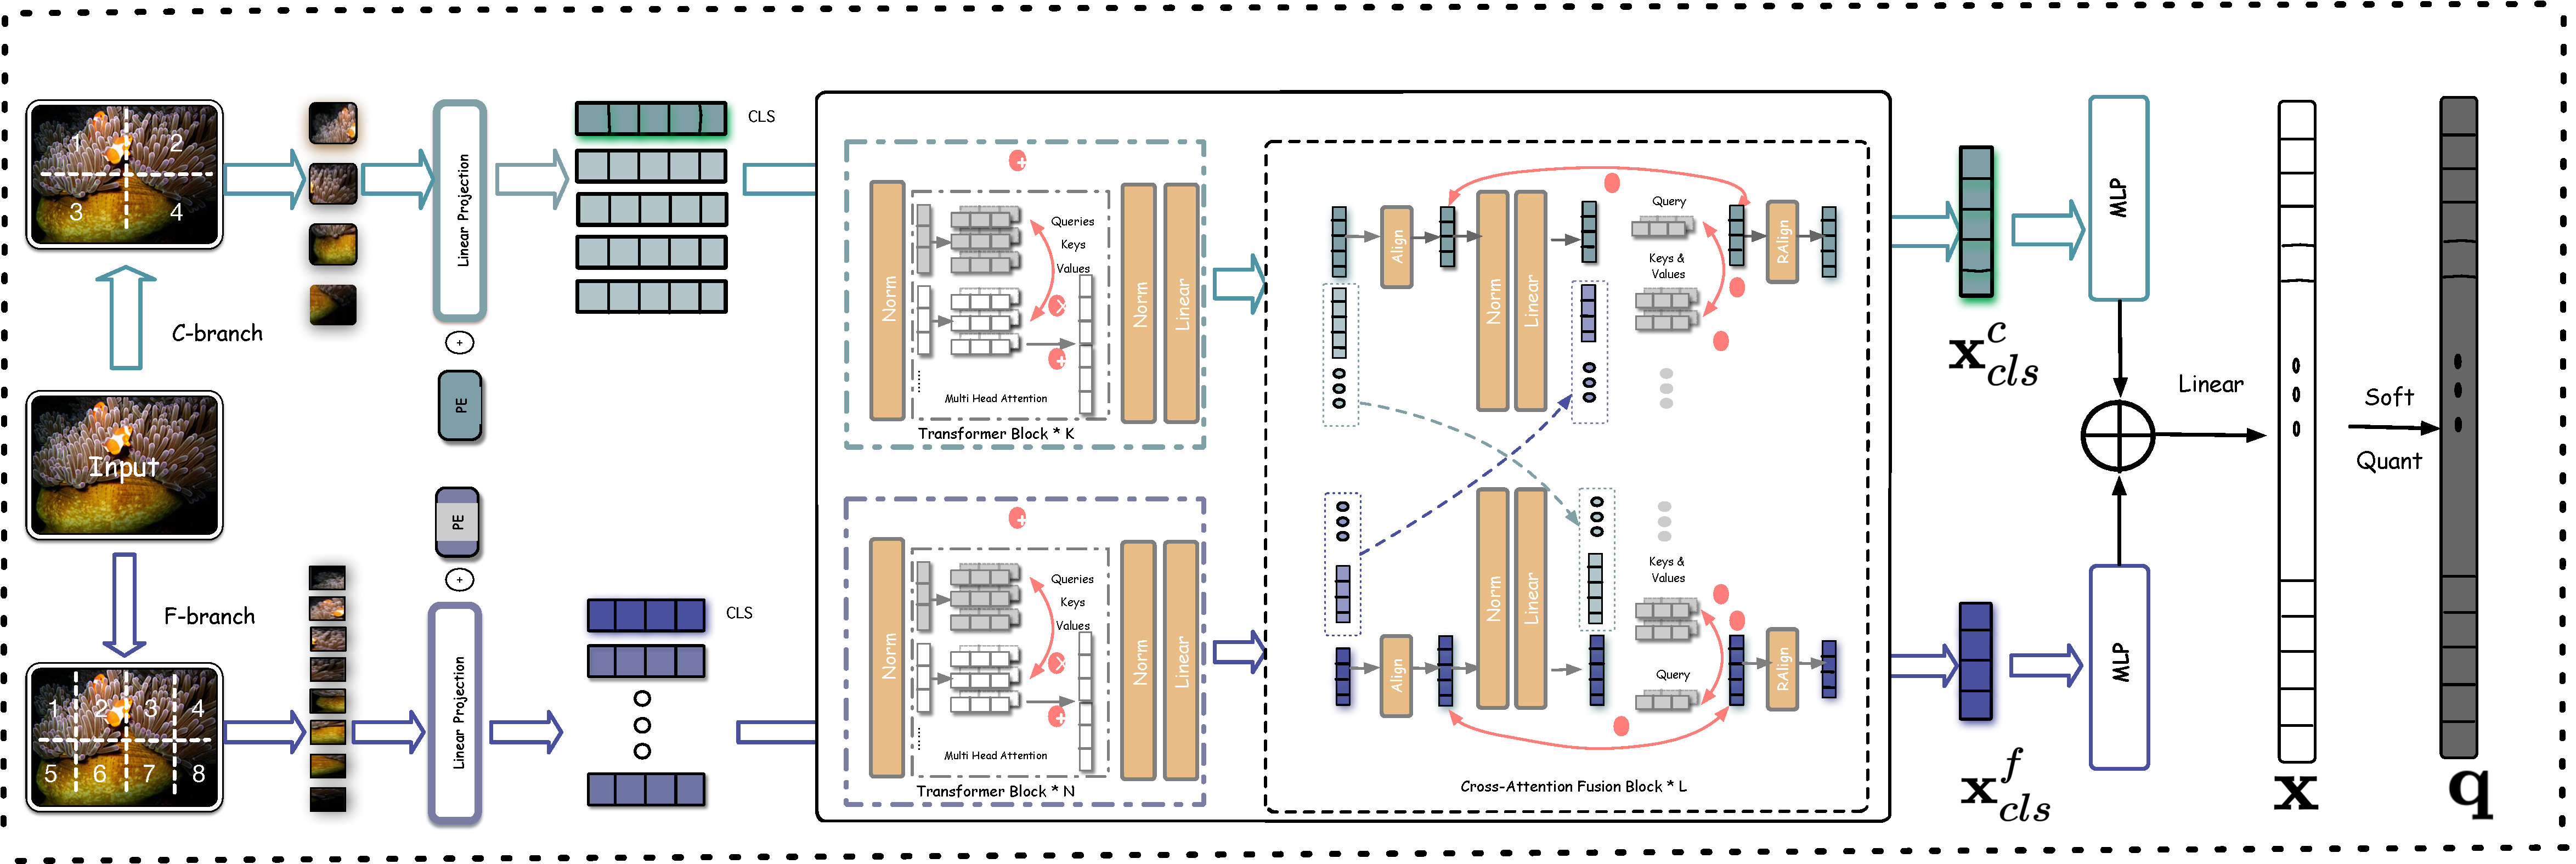
\includegraphics[width=15cm]{05/main1.pdf} \\
  \bicaption[基于Vision Transformer的深度乘积量化框架]
    {基于Vision Transformer的深度乘积量化框架~\textbf{APQFormer}。框架的左边是基于双支的Vision Transformer架构用于多尺度细粒度特征提取。右边包含一个软乘积量化层用于进行乘积量化学习。}
    {The detailed architecture of the proposed \textbf{APQFormer} for deep product quantization learning. The left part of the figure illustrates the dual-branch vision transfomer-based network for fine-grained feature learning. The right part exibits the soft  quantiation layer for product quantization learning. }
 \label{fig:mainapq}
\end{figure} 


乘积量化(Product Quantization, PQ)将原有的特征空间分解成$\mathbf{M}$个子空间。随后, 每一个子空间被量化成$\mathbf{K}$个组(sub-codewords)~\cite{klein2019end}, 这样总共生成了$\mathbf{M}$本 sub-codebook以及$\mathbf{M}\times\mathbf{K}$个sub-codewords。 对于一个输入向量$\mathbf{x} \in  \mathbb{R}^{MD}$, 它先被分割成$\mathbf{M}$个属于 $\mathbb{R}^D$空间的子向量, $ \mathbf{x} =  [\mathbf{x}_1,\mathbf{x}_2,...,\mathbf{x}_M]$。随后, 它通过对每个子向量进行向量量化编码得到一个紧凑的哈希码 $z_x \in \{0,1\}^{M. \log_2{K}}$。这个哈希码是由$\mathbf{M}$组$\log_2{K}$位的短哈希码拼接而成。对于第$m$个$\log_2{K}$的短哈希码, 它代表着输入的第$m$个子向量对应的sub-codeword在第$m$本sub-codebook中的索引,  $i \in \{0,\cdots,K-1\}$。\par
基于深度乘积量化的检索方法通常包含两个阶段: (1) 基于深度卷积神经网络,例如AlexNet,的特征学习。(2)基于上一阶段学习到的特征向量的乘积量化学习。以往的先驱算法通常采取一个二阶段的学习方法~\cite{yue2016deep, liu2018deep, cao2017deep}。第一阶段一般通过监督学习的方法来学习生成有判别性的特征向量。在第二阶段, 通常使用无监督的K-means聚类方法来学习每个sub-codebook中的所有sub-codewords。 尽管这些方法取得了一定程度上的成功, 基于无监督的量化在乘积量化生成codewords的阶段忽略了监督信号的作用, 从而只能达到次优的性能。 \par
\begin{figure}[!htp]
  \centering
  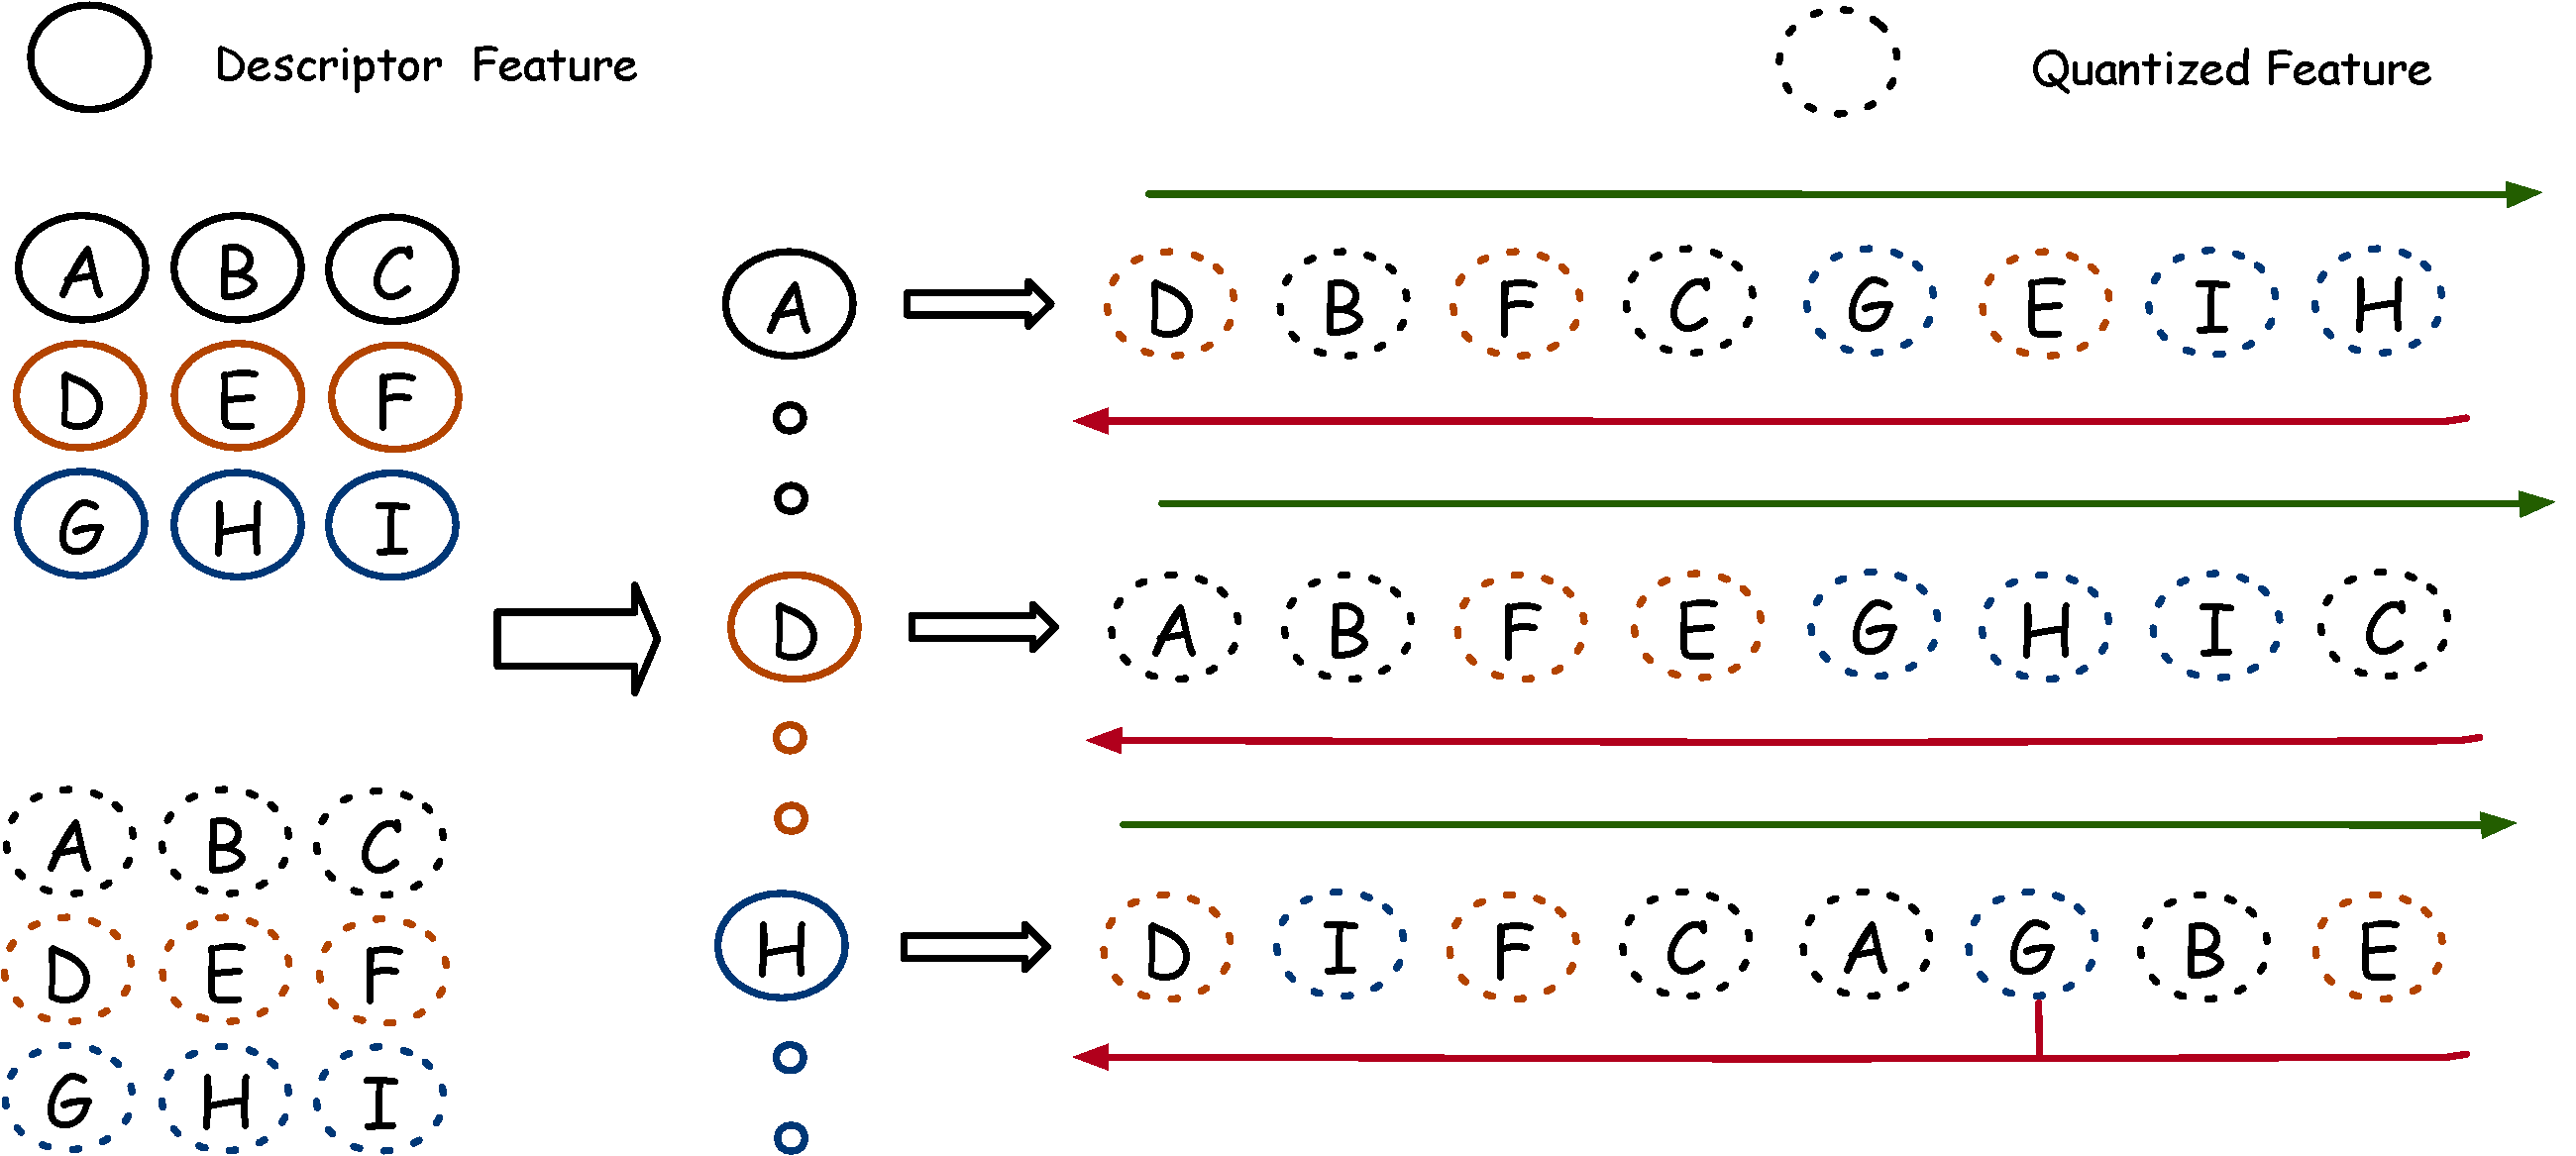
\includegraphics[width=15cm]{05/main2.pdf} \\
  \bicaption[直接优化平均精度\textbf{AP}的量化损失函数]
    {平均精度量化损失函数-\textbf{APQ}的描述。}
    { The description of the average product quantization (\textbf{APQ}) loss.}
 \label{fig:mainapq1}
\end{figure} 

我们通过合并以上两个阶段, 将乘积量化融入到监督学习框架中从而端到端的进行乘积量化学习。受以往工作~\cite{jang2020generalized, yu2018product, dosovitskiy2020image, chen2021crossvit}等的启发, 我们提出一个基于双支Vision Transformer的乘积量化神经网络如图~\ref{fig:mainapq}所示。 其通过两个不同的分支对不同的图片大小分块学习融合的多粒度特征, 同时通过一个可以训练的乘积量化层来对特征向量进行量化。对于相似度保持的量化学习, 迄今为止有不少基于排序损失设计的量化损失函数, 例如基于三元组的损失函数~\cite{jegou2010product}以及n元组的损失函数~\cite{jang2020generalized}。然而, 如Revaud所示~\cite{revaud2019learning}, 优化基于排序损失的目标函数并不能保证优化我们的最终评估指标~\textbf{mAP}。同时, 这些量化损失函数需要机器学习从业人员手工对高敏感的超参数进行微调, 例如三元损失函数中的边界超参数~\cite{cakir2019deep}。为了解决以上的问题, 我们设计了一个新型的量化损失函数-平均精度量化损失(\textbf{APQ})-来进行相似度保持的端到端的监督乘积量化学习, 如图~\ref{fig:mainapq1}。平均精度(Average Precision, AP)的计算是不可导的, 非常难通过传统的基于梯度的框架进行优化。我们通过histogram binning 的方法重新定义\textbf{AP}的计算, 同时采取线性插值的方法来将不可导的直方图桶计数的问题转化成为一个可导的连续性的目标函数。具体来说, \textbf{APQ}通过将未量化的特征向量当作查询向量, 量化后的向量当作被检索的向量。在得到一个返回的检索向量排序集后, 通过在这个返回的列表计算一个\textbf{AP}的可梯度优化的替代目标来进行优化。通过这个\textbf{APQ}新型的度量学习目标函数, 本章提出的框架可以直接可以直接学习到紧凑的乘积量化编码并且这种编码在评估指标\textbf{mAP}上是最优的。 总而言之, 本章的主要工作与贡献如下:
\begin{enumerate}
    \item 本章设计了第一个完全基于Transformer的深度乘积量化框架来进行大规模的图像检索-\textbf{APQFormer}。其包含了一个新型的双支Vision Transformer的乘积量化网络来进行端到端的多尺度特征学习以及一个新型的量化损失函数用于监督进行相似度保留学习。
    \item 本章提出了一个新型的量化损失函数, 平均精度均值量化损失(\textbf{APQ})来进行语意保留的度量学习。它直接在检索返回的量化后的特征向量列表上优化平均精度(\textbf{AP})的连续的可导的替代目标函数。通过最小化这个损失函数, 我们可以直接优化在测试阶段使用乘积量化使用非对称的检索策略进行检索时候的评估指标(\textbf{mAP} )。
    \item 本章在两个标准的公共大规模检索数据集上进行了不同哈希长度下的检索实验-\textbf{CIFAR-10}和\textbf{IMAGENET}。实验结果表明本章提出的框架-\textbf{APQFormer}-可以取得比先进算法显著的性能提升, 证实了算法的有效性。
\end{enumerate}

\section{相关工作}
早期的针对高效的图像检索工作依赖于手工提取的特征 (例如, SIFT~\cite{lowe2004distinctive}) 来得到刻画图片的特征用于后续的哈希码的生成。这种方法一般被称作是浅哈希方法。典型的工作包括无监督的浅层哈希方法 (\textbf{SH}~\cite{weiss2008spectral}, \textbf{ITQ}~\cite{gong2012iterative} 和\textbf{MLH}~\cite{norouzi2011minimal}) 和有监督的浅层哈希方法 (\textbf{KSH}~\cite{liu2012supervised} 和 \textbf{BRE}~\cite{kulis2009learning})。确切地说, \textbf{SH}~\cite{weiss2008spectral}提出最小化图片对之间的带权的汉明距离。同时, \textbf{ITQ} 通过基于在手工提取的特征上最小化量化误差来最小化将实值特征向量二值化的信息损失。为了使用监督标签来获得更好的语义保留的效果,~\textbf{KSH}~\cite{liu2012supervised}和\textbf{BRE}~\cite{kulis2009learning}提出在核空间进行相似度语义保留的哈希学习。尽管这些方法取得了一定程度上的成功, 但是由于手工提取的特征很难准确的保留图像中的语义信息, 这些方法只能取得次优的性能。\par
靠虑到于这一个主要的限制点, 利用卷积神经网络(例如, AlexNet~\cite{alexnet}, ResNet~\cite{he2016deep})来进行端到端的特征提取的深度哈希算法开始获得科研人员的大量关注。它们一般可以被分为两个类别: (1)深度汉明码哈希方法 和深度乘积量化的方法。深度汉明哈希的方法通过深度神经网络学习到一个哈希函数将图片从原本的空间映射到一个汉明空间, 并且在汉明空间中保持原图片的相似性。典型的例子包括\textcircled{1}单点哈希方法~\cite{lin2015deep}, \textcircled{2}成对哈希方法~\cite{liu2016deep,cao2017hashnet,cao2018deep,fan2020deep} \textcircled{3} 三元组哈希方法~\cite{lai2015simultaneous,wang2016deep,li2019triplet}。\textcircled{1}单点哈希方法主要包含: Lin~\cite{lin2015deep}是第一批探究深度卷积神经网络在哈希学习中的工作。通过使用在ImageNet上预训练的AlexNet模型在哈希的数据集上进行分类微调, 然后采取分层次的方法进行检索。\textcircled{2}成对的哈希方法主要有: Liu 和 Cao等人\cite{liu2016deep,cao2017hashnet}提出基于一个贝叶斯学习的框架基于成对的图片输入以及其对应的图片对之间的相似度标签来进行度量学习, 以及对应的量化损失函数来降低连续性的哈希向量和二进制哈希码之间的信息差。Cao~\cite{cao2018deep}提出了一个基于柯西分布作为概率输出函数, 使用成对的交叉熵损失进行度量学习来学习紧凑的哈希编码。 \textcircled{3}三元组的哈希方法通常是使用三元损失函数进行相似度保留的度量学习。2015年, Lai等人~\cite{lai2015simultaneous}提出第一个基于三元损失函数的排序损失进行哈希学习, 并且通过一个divide-and-conquer的模块生成哈希码并且降低哈希码的冗余。然而以上基于排序损失改进的哈希算法都是在优化essential loss~\cite{liu2011learning}, 这是平均精度均值\textbf{mAP} 的一个上界。因此, 优化这些目标函数不一定能够保证可以优化最终的评估指标\textbf{mAP}。 为了解决这个问题, He等人~\cite{he2018hashing}提出一个tie-aware的哈希框架将汉明距离的整数性质考虑进其中, 同时通过直接优化\textbf{mAP}以及归一化折损累积收益~\textbf{NDCC}来进行端到端的哈希训练。\par
由于二进制哈希码的生成一般需要使用一个不能导的\textit{Sign}激活函数来进行量化导致无法端到端通过梯度下降的方法进行训练, 现阶段的``深度汉明哈希方法''通常采取持续放松~\cite{liu2016deep}的方法来绕过这一难题。它们采取的做法是通过在训练阶段优化一个放松的连续的可导的目标函数, 然后在测试阶段使用\textit{Sign}函数进行二值化生成二进制的编码。然而由于放松后的连续性的目标函数已经远离了原始的离散优化的目标函数, 这通常会导致次优的性能。``深度乘积量化''方法通过使用乘积量化将原始的连续性高维向量量化成二进制编码可以有效的解决上述的问题。\textbf{DQN}\cite{yue2016deep}是第一个探究乘积量化~\cite{jegou2010product,ge2013optimized,zhang2014composite}在深度哈希上应用的工作。它采取了一个成对的训练策略基于余弦损失函数来学习实值的特征向量以及一个随后的量化损失函数来进行无监督的乘积量化学习。 Liu等人随后提出了一个三元量化方法~ \cite{liu2018deep}, 通过提出一个组内最难三元组生成方法动态在每个批次的输入组建困难的三元组, 然后使用三元损失函数进行度量学习。然而这样的方法有一个关键的缺陷, 从而导致了性能的下降。由于基于这种机制的乘积量化的过程和深度神经的监督训练过程分离开来, 并且是基于无监督的k-means聚类算法来实现。由于基于k-means的聚类的乘积量化过程无法使用监督的标签进行训练, 也无法反馈调整前一阶段的特征学习的效果, 这种模式的性能大大的受限。因此, Yu, Klein 以及Jang等人~\cite{yu2018product, klein2019end,jang2020generalized}提出将乘积量化融合进入端到端的深度神经网络监督训练中, 通过\textit{Softmax}来在训练阶段接近乘积量化的效果。\par
Transformer最初是由\textbf{Google}公司提出在自然语言处理替代基于编码器和解码器的神经网络架构~\cite{vaswani2017attention}。一经提出, \textbf{Transformer}就迅速成为了自然语言处理领域的标准主干神经网络框架。2020年末, \textbf{Google} 又进一步提出Vision Transformer (ViT) 将Transformer引入到计算机视觉领域, 从而成为了卷积神经网络的一个极强的替代神经网络模型。从此, 基于Vision Transformer的计算机视觉模型开始迅速发展, 在各个计算机视觉任务上展现出比卷积神经网络更优越的性能。DeiT~\cite{touvron2021training}~是一个Transformer可以在中等大小的数据集上进行预训练并且取得较有的性能。DeiT通过使用CNN的输出当做一个教师模型, 通过蒸馏学习(Distillation Learning)来帮助训练自身的Transformer架构。在输入的嵌入表征前, 它们添加了一个蒸馏表征, 然后通过交叉熵损失和蒸馏损失进行训练。随后 Token-to-Token (T2T) Vision Transformer~\cite{yuan2021tokens}递归的将临近的token融合成一个token来降低序列的长度并且对于空间中的较远的联系进行建模。 Liu等人\cite{liu2021swin} 提出了Swin Transformer, 一个基于Vision Transformer的变种。其通过提出Window Self Attention 将自注意力的计算限制在固定大小的窗口内从而极大的降低计算复杂度, 使得Vision Transformer可以处理更大的现实视觉任务。 He 等人\cite{he2021transreid}提出了第一个完全基于Transformer的行人重识别框架, 并且在多个行人重识别以及车辆重识别领域获得了超越当前最先进的基于卷积神经网络的重识别框架的性能。Wang等人 \cite{wang2021pyramid}提出一个Pyramid Transformer来进行密集预测。 Cheng等人\cite{wang2021crossformer}提出了一个跨尺度的Transformer来学习更加细粒度的图像特征来进行图像分类任务。 随后, Chen~\cite{chen2021regionvit}提出一个新型的 region-to-local 注意力机制来替代原ViT中的自注意力机制。为了学习到更多的细粒度特征, Chen\cite{chen2021crossvit} 设计了一个双支的Transformer框架来学习图像中不同尺度的特征。\par
在本章中, 受以往的工作的启发 \cite{chen2021crossvit,cakir2019deep,revaud2019learning}, 我们提出了一个平均精度均值量化Transformer (Avereage Precision Quantization Transformer, \textbf{APQFormer})。具体来说, 受Chen和Yu的工作启发\cite{chen2021crossvit,yu2018product}我们设计了一个双支 Vision Transformer 量化神经网络来进行端到端的特征学习。对于相似度保留的度量学习, 本章采取了和当前的量化损失函数完全不同的策略。我们通过直接优化非对称检索的\textbf{mAP}评估指标来优化整个框架。由于\textbf{mAP} 的计算并不可导, 因此无法通过标准的随机梯度下降算法进行训练学习。He 等人\cite{he2018hashing,he2018local} 展示了通过histogram binning算法\cite{ustinova2016learning}来建立一个近似不可导\textbf{mAP}计算的可导的目标函数。 2018年, He\cite{he2018hashing}提出一个为深度汉明哈希设计的通过优化\textbf{mAP}的框架, 但是并不能适用于乘积量化学习。除此之外, 也有其他的工作基于直接优化这个评估指标进行度量学习~\cite{yue2007support,mcallester2010direct,oh2016deep,henderson2016end}。 Yue 提出通过一个loss-augmented的推断问题~\cite{mcallester2010direct}采取线性支持向量机(Support Vector Machine, svm)来优化\textbf{AP}。Song 等人\cite{song2016training} 随后将这个框架扩展到非线性的模型中。然而, 这些方法需要需要采取一个动态规划的方法, 从而偏离了原先的优化问题本身。随后, 一系列的工作开始\cite{he2018local,henderson2016end,revaud2019learning}通过直接优化基于\textbf{AP}的损失来优化深度神经网络框架分别在面片验证, 目标检测以及图像检索的应用。\par
尽管以上的方法取得了比较惊人的性能, 这些\textbf{AP}的变种, 由于乘积量化一般是通过无监督k-means进行训练,从而并不能直接应用在乘积量化学习中。同时, 乘积量化一般的非对称检索性质也应该被考虑进度量学习之中。本章提出的 \textbf{APQ}量化损失函数是第一个端到端的基于直接优化\textbf{AP}的适用于大规模图像检索的量化损失函数。 
\section{乘积量化的背景}
在本小节中, 我们介绍与乘积量化相关的背景知识, 从而方便理解后续的实现细节。我们先从乘积量化的最初的向量量化开始介绍, 最后介绍乘积量化的基础。
\subsection{向量量化}
乘积量化是向量量化(Vector Quantization, VQ)~\cite{gray1984vector} 的一种变种。 VQ 通过学习来将一个长度为$d$的特征向量$\mathbf{x} \in \mathbb{R}^d$ 映射到\textit{codebook} $\mathcal{C}$中的\textit{codeword} $\textbf{c}$中。映射的函数被正式成为一个量化器(Quantizer):  $\mathcal{Q}(\mathbf{x}) \mapsto \{\mathbf{c}_1,...,\mathbf{c}_N\}$。其中 $N$代表了\textit{codebook} $\mathcal{C}$中\textit{codewords} 的数量。向量量化的目标函数是为了减少量化的误差, 如下式所示:
\begin{equation}
    \label{eq:vq}
      \min E = \frac{1}{N_{D}} \sum_{\mathbf{x}} ||\mathbf{x} - \mathcal{Q}(\mathbf{x}) ||^2_2
  \end{equation}
其中,  $||.||$代表了$l_2$正则化,  $N_{D}$则代表被量化的所有特征的数量。给定一个 \textit{codebook} $\mathcal{C}$ 最小化式子~\ref{eq:vq} 可以得到一个满足 Lloyd 条件的~\cite{gray1984vector}的量化器。Lloyd 条件是指一个向量 $\mathbf{x}$ 应当永远通过量化器$\mathcal{Q}(\mathbf{x})$被映射到\textit{codebook}中$\mathcal{C}$离它最近的\textit{codeword}上。通常, \textit{codebook} $\mathcal{C}$中的\textit{codewords}一般由无监督k-means算法通过预先定义的聚类数$N$来生成。
\subsection{乘积量化}
当\textit{codeword}$\mathbf{c}$需要从一个有限数量的\textit{sub-codebook}的笛卡尔乘积中取时~\cite{ge2013optimized}, 优化公式~\ref{eq:vq}会就会得到乘积量化算法~\cite{jegou2010product}。\par
正式来说, 对于一个输入的特征向量$\mathbf{x} \in \mathbb{R}^d$, 我们将其分割成$M$个子向量$x^s$, 其中每一个子向量$x^s$ 的维度为$\frac{d}{M}$。我们将$\mathbf{x}$ 视为 $M$个子向量的和 $\mathbf{x} = [x^s_1,...,x^s_m,...,x^s_M]$。\textit{Codebook}$\mathcal{C}$中的每一个\textit{codeword} 都是$M$个 $M$ \textit{sub-codewords}的拼接: $\mathbf{c} = [c^s_1,...,c^s_m,...,c^s_M]$ 和  $\mathcal{C} = [\mathcal{C}^s_1,...,\mathcal{C}^s_m,....\mathcal{C}^s_M ]$。对于每一个\textit{sub-codebook} $\mathcal{C}^s_m$, 一般在子向量空间$x^s_m$中采取无监督k-means聚类生成。乘积量化的量化器可以用如下的公式所表示:
\begin{equation}
    \begin{aligned}
    \mathcal{Q}(x) = [\mathcal{Q}^1_{hard}(x^s_1),...,\mathcal{Q}^m_{hard}(x^s_m),...\mathcal{Q}^M_{hard}(x^s_M)]
    \end{aligned}
    \end{equation}
  其中 $\mathcal{Q}_m$ 是子空间 $\mathbf{x_m}$的量化器, 并且可以被表示为:
    \begin{equation}
    \label{eq:pq1}
    \begin{aligned}
    &\mathcal{Q}^m_{hard}(\mathbf{x}_m) = \argmin_{(c^s_m)_k} ||\mathbf{x}_m^s - (c^s_m)_k ||^2_2  \\
    &\text { s.t.}  \quad k \in  \{i\}_{i=1}^{i=K}
    \end{aligned}
    \end{equation}
其中$K$是在\textit{sub-codebook}$\mathcal{C}_m^s$中的 \textit{sub-codewords}的数量。乘积量化的最大贡献是由于最终的\textit{codewords}数量是各个\textit{sub-codebook}的笛卡尔乘积, 这样可以生成大量的\textit{codewords}。例如, 如果每个\textit{sub-codebook}是由$K$ \textit{sub-codewords}组成, 则其笛卡尔乘积的结果组成的最终\textit{codebook} $\mathcal{C}$ 包含 一共$K^M$个\textit{codewords}。这对于给予向量量化的方法来说是无法做到的。
\section{基于Vision Transformer的量化方法}
\subsection{本章主要符号定义以及问题定义}
在本章中, 我们使用书法大写字母 (Calligraphic Uppercase), 例如 $\mathcal{H}$ 来表示映射函数。我们使用粗体大写字母 (Bold-face Uppercase) 如 $\mathbf{T}$ 来代表集合. 粗体小写字母如 $\mathbf{b}$在全章中代表向量。我们使用斜大写字母 (Italic Uppercase)来代表图片, 如 $\textit{I}$。 同时, 在全章中, sign激活函数直接由 $\textit{sign}$ 来表示。\par
\textbf{问题定义:} 假设我们有一个训练数据集 $\mathbf{I} = \{ I_i\}_{i = 1}^N$ 和一个对应的标签集合$\mathbf{Y} = \{\mathbf{y}_i\}_{i=1}^N$。我们定义了一个对于成对的图片的相似度函数$\mathcal{S}: (Y_i,Y_j) \mapsto \{0,1\}$。 如果 $y_i y_j^T > 0$ 则$\mathcal{S}(y_i,y_j) = 1$, 否则 $\mathcal{S}(y_i,y_j) = 0$。深度乘积量化是要通过深度神经网络学习一个复合量化器
$f_{\Theta}: I \rightarrow \mathbf{b} \in \{ 0,1 \}^B$, 其中$\Theta$是神经网络中可以学习的参数。深度乘积量化的目标是将图片$\it{I}$映射到二进制量化编码同时最小化量化误差。
\subsection{双支Vision Transformer乘积量化网络}
我们的乘积量化网络是在由Chen等人提出\cite{chen2021crossvit}的Vision Transformer上构造。它包含了两个分支来学习两个尺度的特征以及一个跨尺度注意力融合模型来融合来自两个分支的特征。另外, 它还包含一个可以训练的乘积量化网络层来进行端到端的乘积量化。 \par
\begin{figure}[!htp]
  \centering
  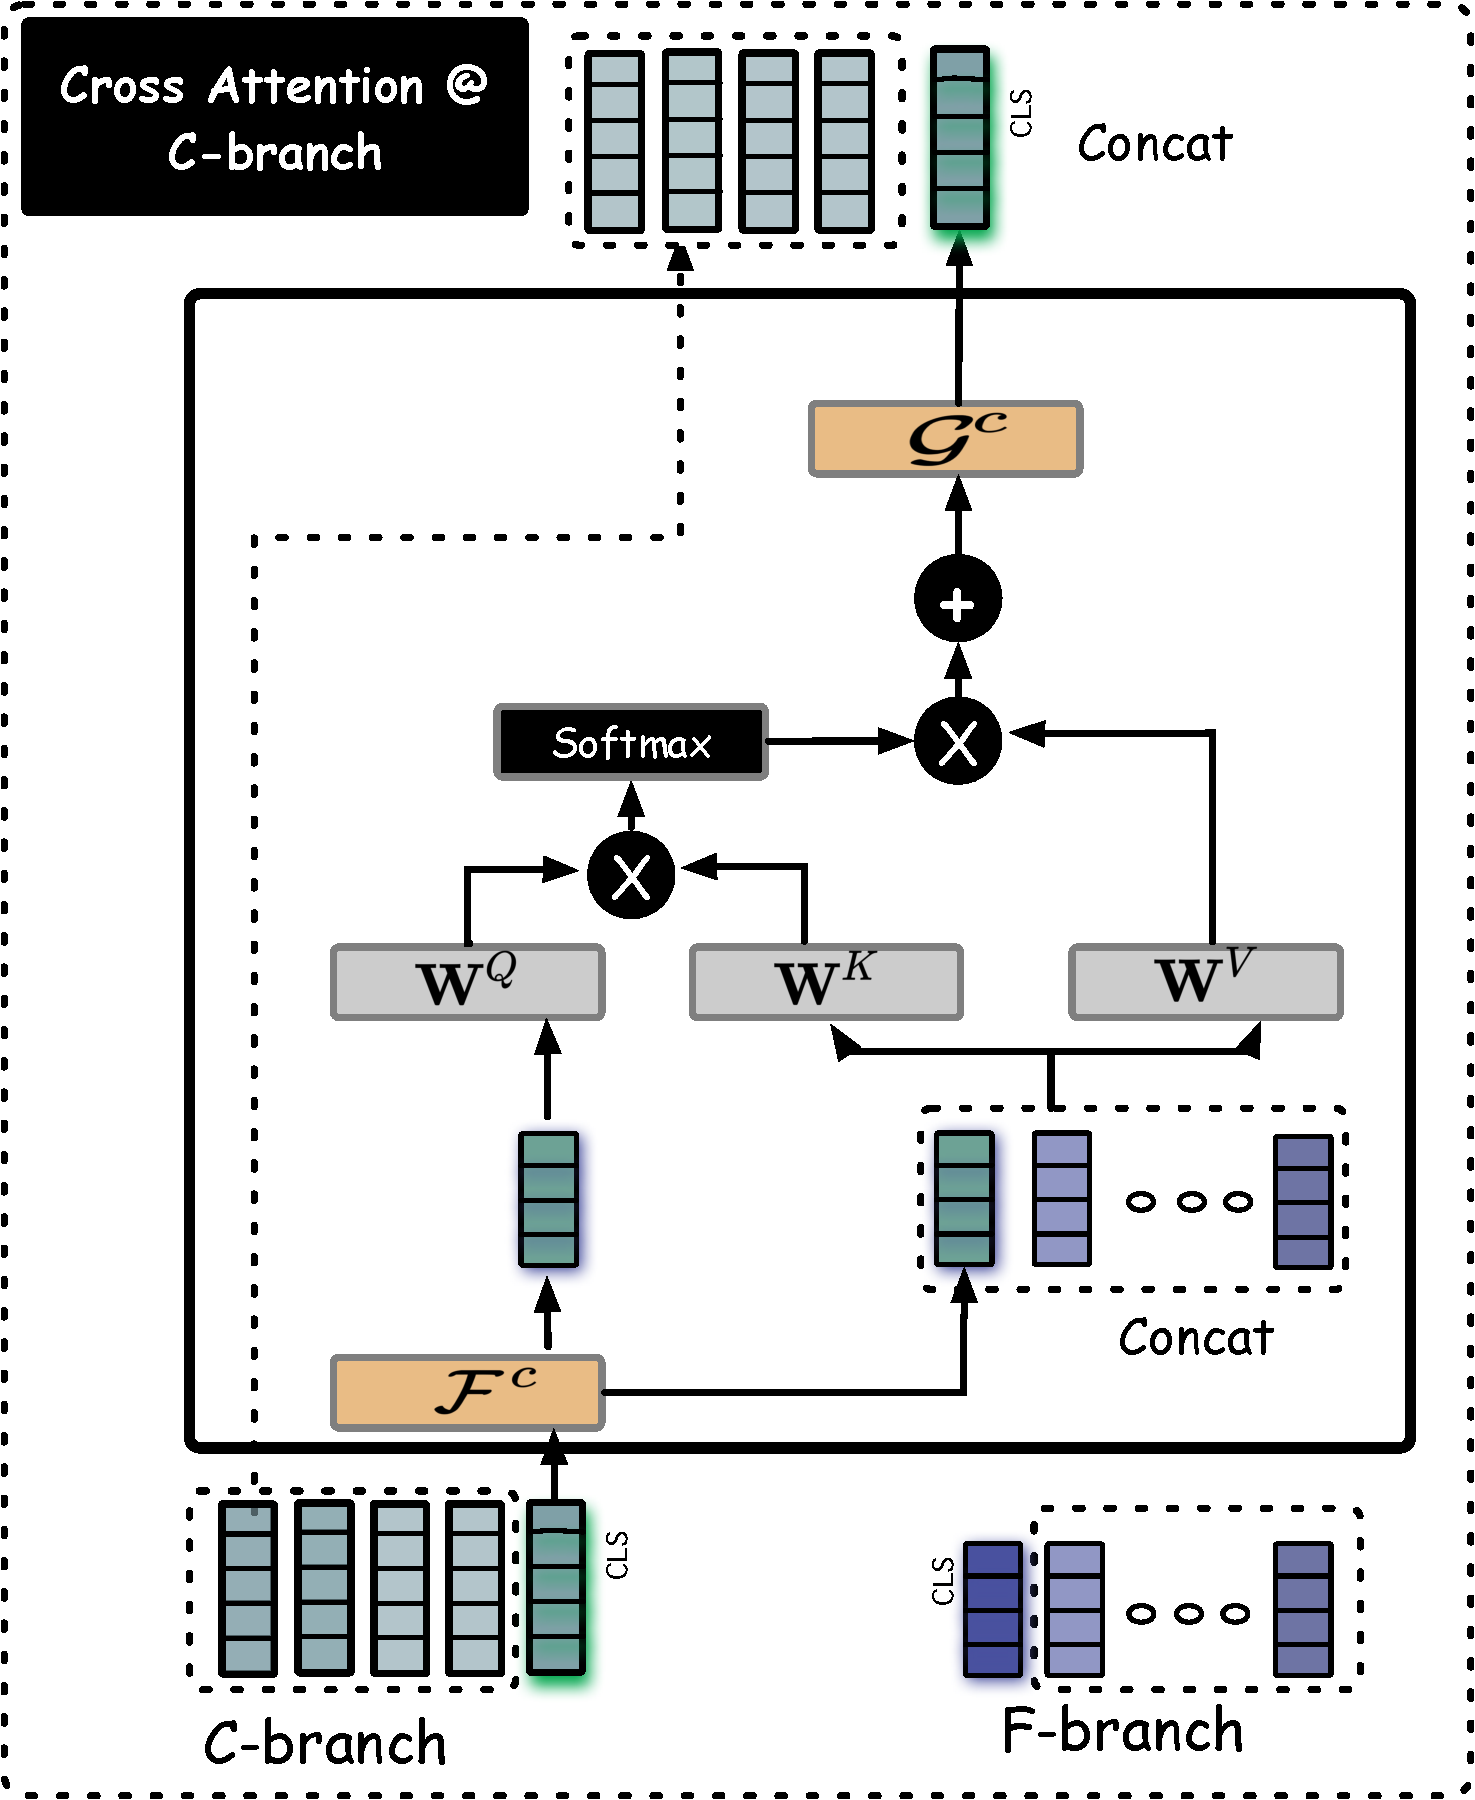
\includegraphics[width=8cm]{05/main3.pdf} \\
  \bicaption[跨尺度特征学习]
    {\textbf{C-branch}的跨尺度自注意力机制。}
    { The cross attention mechanism for the \textbf{C-branch}.}
 \label{fig:mainapq3}
\end{figure} 



\textbf{传统Vision Transformer的背景知识:} Vision transformer (ViT)~\cite{dosovitskiy2020image}通过先将图片分割成一个块序列, 随后将二维的拉平成一个向量, 通过线性映射来将它们映射成token $\mathbf{x}_{patch}$。我们在序列的头部额外添加一个用于分类 \textit{CLS}的token $\mathbf{x}_{cls}$, 用于学习作为分类的表征。类似于传统的Transformer, ViT 对每一个token添加了对应的位置编码来学习二维位置信息。随后, 所有的token被输入进传统的Transformer编码器, 此编码器一般包含多个block。每一个block包含一个多头注意力机制(Multi-headed Self-attention, MSA)以及一个全连接层。同时, 在每一层前都会进行层标准化的操作, 并且在每一层后会使用残差连接。ViT的第一层的输入 $\mathbf{x}_0$以及第$i$层的计算可以用公式写为:
\begin{equation}
    \begin{aligned}
    &\mathbf{x}_{0}=\left[\mathbf{x}_{cls} \| \ \mathbf{x}_{\text{patch}}\right]+\mathbf{x}_{\text {pos }} \\
    &\mathbf{y}_{i}=\mathbf{x}_{i-1}+\mathbf{MSA}\left(\mathbf{LN}\left(\mathbf{x}_{i-1}\right)\right) \\
    &\mathbf{x}_{i}=\mathbf{y}_{i}+\mathbf{FFN}\left(\mathbf{LN}\left(\mathbf{y}_{i}\right)\right)
\end{aligned}
\end{equation}
其中$x_{cls} \in \mathbb{R}^{1\times C}$ , $x_{patch} \in \mathbb{R}^{N\times C}$ and $x_{pos} \in \mathbb{R}^{(1+N) \times C}$分别是 \textit{CLS} token, 图片块 token以及每一个token的位置编码。而 $N$ 和 $C$则是图片块的数量以及嵌入编码的维度。 \par
\textbf{双支网络特征学习}
对于Vision Transformer而言, 切割的图片块的大小和模型最后的准确性以及计算复杂度紧密相关。一般来说, ViT在图片块切割较小数量较多的情况下可以学习到更加细粒度的特征, 从而取得更加优异的性能。但是, 这样的切割通常会导致显著的内存消耗增长以及计算量的增长。如Chen等人\cite{chen2021crossvit}指出, 当图片快大小为$16$时, ViT的性能可以超越图片块为$32$ 的情况接近$6\%$。 但是同时, 它也需要接近4倍的计算开销。 为了在获得更加细粒度的特征表示的同时防止模型复杂度的爆炸性增长, 我们采用了一个双支的ViT, 如图~\ref{fig:mainapq1}所示。具体来说, 在多尺度Transformer内部由下面两个分支: (1)  \textbf{C-Branch}: 是一个采取大图片块切割策略的分支, 用于学习粗粒度的特征。 (2) \textbf{F-branch}: 是一个采取较小图片块的分支, 用于学习更加细粒度的特征。 每一个分支后都是使用得标准的Transformer 编码器。 为了平衡两个分支的计算, 我们通常对于\textbf{C-Branch} 会采取较多的block, 而对于\textbf{F-branch}则会使用较少的。\par
\textbf{跨尺度特征融合} \quad
由于本章设计的目标是为了学习多尺度的判别性特征, 我们需要充足有效的融合来自由两个分支的特征。为了实现这一目的, 我们采取了额外的跨尺度特征融合策略使得每一个分支可以和另一个分支交换信息。具体做法是, 每一个分支的\textit{CLS} token用来和另一个分支的除\textit{CLS}外的token进行交互, 来学习到另一个分支信息。如图~\ref{fig:mainapq3}所示, 以\textbf{C-branch}为例, 为了使\textbf{C-branch} 的\textit{CLS}token包含来自\textbf{F-branch}的信息, 我们将\textbf{C-branch} 的\textit{CLS} token和 来自\textbf{F-branch}的块token进行拼接:
\begin{equation}
    \mathbf{x}^{\prime c}=\left[\mathcal{F}^{c}\left(\mathbf{x}_{c l s}^{c}\right) \ || \ \mathbf{x}_{\text {patch }}^{f}\right]
\end{equation}
其中$\mathcal{F}^c$ 是一个线性映射, 用于对齐两个分支的特征的维度。随后, 我们对\textit{CLS}向量$\mathbf{x}_{cls}^c$使用交叉注意力(Cross-attention, CA)来生成一个融合的特征。通过将 $\mathbf{x}_{cls}^c$ 作为唯一的query向量, 这个注意力可以生成一个新的 \textit{CLS} token, 其充分融合了来自\textbf{F-branch}的细粒度特征。  \textbf{CA} 以及对应的多头交叉注意力(Multi-headed Cross Attention, MCA)如下式所示:
\begin{equation}
    \begin{aligned}
    \textbf{ MCA }(Q, K, V) &=\text { concat }\left(\textbf{head}_{\ 1}, \ldots, \textbf{head}_{\ \mathrm{h}}\right) W^{O} \\
    \text { where \quad \textbf{head}}_{\ \mathrm{i}} &= \textbf{CA }\left(Q \mathbf{W}_{i}^{Q}, K \mathbf{W}_{i}^{K}, V \mathbf{W}_{i}^{V}\right) \\
    \textbf{ CA }(\textbf{q}, \textbf{k}, \textbf{v})  &= \operatorname{softmax}\left(\frac{\textbf{q} \textbf{k}^{T}}{\sqrt{d}}\right) \textbf{ v}
    \end{aligned}
\end{equation}
其中$Q = \mathbf{x}_{cls}^{c}$, $K = \mathbf{x}^{\prime c}$ 并且 $V = \mathbf{x}^{\prime c}$。$\mathbf{W}^Q_i$,~$\mathbf{W}^K_i$,~$\mathbf{W}^V_i \in \mathbb{R}^{d/h}$是可以训练的注意力的参数矩阵。 $d$ 和 $h$则是嵌入的维度以及多头注意力的头数。随后, 对于来自粗粒度分支\textbf{C-branch}的 $\mathbf{x}^c$ 的跨尺度特征融合则可以表示如下:
\begin{equation}
    \begin{aligned}
\mathbf{y}_{c l s}^{c} &= \mathcal{F}^{c}\left(\mathbf{x}_{c l s}^{c}\right)+\textbf{MCA}\left(\textbf{LN}\left(\left[\mathcal{F}^{c}\left(\mathbf{x}_{c l s}^{c}\right) \ \| \ \mathbf{x}_{\text {patch }}^{f}\right]\right)\right) \\
\mathbf{z}^{c} &=\left[\mathcal{G}^{c}\left(\mathbf{y}_{\text {cls }}^{c}\right) \ \| \ \mathbf{x}_{\text {patch }}^{c}\right]
\end{aligned}
\end{equation}
其中 $\mathbf{z}^c$是跨尺度特征融合的输出而$\mathcal{F}^c$ and $\mathcal{G}^c$则是为了对其两个分支的维度的一个前向线性映射和一个反向线性映射。\par
\textbf{可训练的乘积量化网络层}\quad
在Transformer网络的最终, 我们通过融合来自两个分支的 \textit{CLS} token得到了一个最终的特征向量 $\mathbf{x}$。在两个分支的输出均使用线性映射来对齐两个分支的特征维度:
\begin{equation}
    \mathbf{x} = \mathcal{F}_{ln}^c(\mathbf{x}^c_{cls}) + \mathcal{F}_{ln}^c(\mathbf{x}^f_{cls}) = (\mathbf{x}^c_{cls} W_c^T + \mathbf{b}_c) + ( \mathbf{x}^f_{cls} W_f^T + \mathbf{b}_f)
\end{equation}
其中$ \mathbf{x}$是需要被量化的特征向量。$W_c \in \mathbb{R}^{L \times d^c }$ 和  $W_f \in \mathbb{R}^{L \times d^f}$ 则是两个分支的线性映射的权重矩阵。而 $\mathbf{b}_c, \mathbf{b}_f \in \mathbb{R}^{L}$则是对应的偏差参数。$d^c$ 和 $d^f$是  \textbf{C-branch} 和 \textbf{F-branch}的嵌入的维度。 传统的使用 $\argmin$的量化方法, 如下式~\ref{eq:soft}所示, 是不可导的。为了将乘积量化的过程融合进Transformer神经网络架构进行端到端的基于梯度下降的学习, 受这些工作\cite{arandjelovic2016netvlad,yu2018product}的启发, 我们观察到下面的等式:
\begin{equation}
    \label{eq:soft}
    \begin{aligned}
    \mathcal{Q}_{soft}\left(\mathbf{x}_{m}\right) &=\lim _{\gamma \rightarrow+\infty} \sum_{k} \frac{e^{-\gamma\left\|\mathbf{x}_{m}-(z_m^s)_k\right\|_{2}}}{\sum_{k} e^{-\gamma\left\|\mathbf{x}_{m}-(z_m^s)_k\right\|_{2}}} (z_m^s)_k \\
    & = \argmin_{(z^s_m)_k} ||\mathbf{x}_m^s - (z^s_m)_k ||_2^2  \\
    &\text { s.t.}  \quad k \in  \{i\}_{i=0}^{i=K-1}
    \end{aligned}
\end{equation}
当 $\gamma \rightarrow+\infty$时,  第$m$个子向量 $x_m$被量化到在第$m$本\textit{sub-codebook}  $\mathcal{Z}_m^s$ 中最近的\textit{sub-codeword}。其中$K$ 是 $\mathcal{Z}_m^s$中 \textit{sub-codeword}的数量。\par
基于这些发现, 我们设计了本章的软量化器如下:
\begin{equation}
    \mathcal{Q}_{soft}(\mathbf{x_m}) = \sum_{k} \frac{e^{-\gamma \mathcal{D}_E(\mathbf{x}_{m},(z_m^s)_k)}}{\sum_{k} e^{-\gamma \mathcal{D}_E(\mathbf{x}_{m},(z_m^s)_k)}} (z_m^s)_k 
\end{equation}
其中$\mathcal{D}(x,z)$是欧式距离函数。 本章采取一个较大的$\gamma$来使得\textit{softmax}函数逼近原先的\textit{argmin}。软量化器$\mathcal{Q}_{\text{soft}}$ 是可导的, 可以直接被嵌入进深度神经网络中进行训练。\par
具体而言, 我们提出一个可以训练的{PQ} \textit{codebook} $\mathcal{Z}$, 其是一个新分配的用于存储$M$\textit{sub-codebooks}的内存。 每一个\textit{sub-codebook}是一个$K \times \frac{L}{M}$的张量。 \textit{codebook}在最初是随机初始化并且设置成可以学习。这样的话可以通过标准的反向传播算法进行优化。因此, 对于一个特征向量$\textbf{x}$, 我们可以由下式获得其量化后的向量$q$:
\begin{equation}
    \label{eq:quantizer}
        \textbf{q} = [\mathcal{Q}^1_{soft}(x^s_1),\cdots,\mathcal{Q}^m_{soft}(x^s_m),\cdots,\mathcal{Q}^M_{soft}(x^s_M)]
    \end{equation}
    
\subsection{平均精度量化学习}
为了进行同时的量化学习以及特征学习, 我们提出了一个新型的直接优化评价指标\textbf{AP}的量化损失函数。 \par
\textbf{针对非对称检索的平均精度}: 由于基于乘积量化的大规模图像检索一般在测试阶段采取非对称的检索策略, 我们将非对称的检索本质嵌入进我们的量化损失函数中。具体来说, 对于一个具有$N+1$张训练图片 $\mathcal{B}=\left\{I_{1}, \ldots, I_{N+1}\right\}$的训练数据集, 以及其对应的监督标签, 我们可以获得一系列的未量化的特征向量$\mathcal{D} = \left\{ \mathbf{x}_{1}, \ldots, \mathbf{x}_{N+1} \right\}$以及
一系列的量化后的的特征向量 $\mathcal{R} = \left\{ \mathbf{q}_1, \ldots, \mathbf{q}_{N+1} \right \}$。我们将每一个未量化的特征向量$\mathbf{x}$当作一个潜在的检索向量,将所有的除检索向量外的对应的量化后的特征向量当成被检索数据库。 随后, 我们根据每一个在$\mathcal{R}$中的向量和 $\mathbf{x}$的欧式距离
$\mathcal{D}_E$ 进行排序, 得到一个排序序列。 平均精度(AP) 则可以用公式描述为:
\begin{equation}
    \mathbf{AP}=\sum_{i=1}^{N} Prec(i) \ \Delta Rec(i)
    \end{equation}
其中 $Prec(i)$ 和 $Rec(i)$ 是在排序序列$i$ 处的准确率以及召回率。其中$\Delta Rec(i) = Rec(i) - Rec(i-1)$。 值得注意的是,  和Cakir等人一致, 为了方便计算, 我们假设 $Rec(0) = Prec(0) =  0$。

\textbf{AP 的近似计算}: 如Boyd所言 \cite{boyd2013area}, 当$|\mathcal{R}^{+}|$ 时, \textbf{AP} 可以被视为准确率-召回率曲线下的面积(~\textbf{AUPR}).
\begin{equation}
    \label{eq:appro}
    \begin{aligned}
    \textbf { AUPR } &=\int_{0}^{1} Prec(Rec) \ d Rec \\
    &=\lim _{\left|\mathcal{R}^{+}\right| \rightarrow \infty} \sum_{i=1}^{N} \operatorname{Prec}(i) \triangle \operatorname{Rec}(i)
    \end{aligned}
\end{equation}
其中$\mathcal{R}^{+} \subset \mathcal{R}$ 是返回的检索集合 $\mathcal{R}$中的和查询图片是属于同一个类别的集合。相对应的$\mathcal{R}^{-}$则是不属于同一个类别的集合。 如 公式~\ref{eq:appro}所示, 准确度(precision)和召回率(recall)可以看做和查询的数据$\mathbf{x}$的欧式距离的函数。这提供了一个新的绕过在\textbf{mAP}中不可导的排序操作的方法。用 $e$来表示查询向量 $\mathbf{x}$ 和被检索数据库中量化后的$\mathbf{q} \in {\mathcal{R}}$ 之间的欧式距离, 其值域为 $\Omega$。 我们可以重新将平均精度~\textbf{AP}用公式描述为:
\begin{equation}
    \label{eq:ap}
     \textbf{AP} = \int_{\Omega}Prec(e) \ dRec(e)
\end{equation}
为了求解式~\ref{eq:ap}, 受cakir的工作\cite{cakir2019deep}的启发, 我们定义了几个概率函数。首先, 让 $\mathcal{E}$ 作为一个随机变量, 代表欧式距离$e$。我们随后定义两个先验分布 $P(\mathcal{R}^{+})$和$P(\mathcal{R}^{-})$, 其中 $P(\mathcal{R}^{+}) = 1 - P(\mathcal{R}^{-})$。$P(\mathcal{R}^{+})$ 表示对于在被检索集合$\mathcal{R}$中, 给定一个查询$\mathbf{x}$ 的正样本的概率。然后, 我们定义随机变量 $\mathcal{E}$ 的概率密度累计函数(Cumulative Distribution Function, CDF)为:$\mathcal{E}$ as $F(e) = P(\mathcal{E} \le e)$。 \par
有了如上的概率密度函数, 我们可以以一种概率密度函数的角度重新定义Precision 和Recall:
\begin{equation}
    \label{eq:bayesian}
    \begin{aligned}
    \operatorname{Prec}(e)=P\left(\mathcal{R}^{+} \mid \mathcal{E}<e\right) 
    &=\frac{F\left(e \mid \mathcal{R}^{+}\right) P\left(\mathcal{R}^{+}\right)}{F(e)} \\
    \end{aligned}
    \end{equation}
\begin{equation}
\operatorname{Rec}(z)=P\left(\mathcal{E}<e \mid \mathcal{R}^{+}\right)=F\left(z \mid \mathcal{R}^{+}\right)
\end{equation}
公式~\ref{eq:bayesian} 可以通过贝叶斯理论来推到得到。通过在式~\ref{eq:ap}中替换这些, 我们可以得到\textbf{AP}的一个表达式如下:
\begin{equation}
    \label{eq:approb}
    \begin{aligned}
    \textbf{AP} &=\int_{\Omega} P\left(\mathcal{R}^{+} \mid \mathcal{E}<e\right) d P\left(\mathcal{E}<e \mid \mathcal{R}^{+}\right) \\
    &=\int_{\Omega} \frac{F\left(e \mid \mathcal{R}^{+}\right) P\left(\mathcal{R}^{+}\right)}{F(e)} p\left(e \mid \mathcal{R}^{+}\right) d e .
    \end{aligned}
\end{equation}
值得注意的是, 我们是用来如下等式:
\begin{equation}
    dP(\mathcal{E} \le e \mid \mathcal{R}^{+}) = P(e \mid \mathcal{R}^{+}) de
\end{equation}
因为\textbf{CDF}的梯度就是对应的概率密度函数\textbf{PDF}。\par 
由于直接优化公式~\ref{eq:approb}是无法求解的, 我们采取有限和(finite sums)问题来近似的解决。具体来说, 我们先$l2$标准化原始的特征 $\mathbf{x}$以及对应的量化后的特征$\mathbf{q}$。通过这种方法, 值域 $\Omega$ 就限定在了 $[0,2]$之间。 随后, 我们将区间$[0,2]$等分成$L$个相同大小的区间, 每个区间中心为
$\{c_1, \ldots, c_L\}$。这样可以生成直方图 $\mathcal{E} = [e_1,\ldots,e_L]$。我们将离散的\textbf{AP}的近似形式表示为:
\begin{equation}
    \label{eq:approap}
    \text { DAP }=\sum_{e \in \mathcal{E}} \frac{F\left(e \mid \mathcal{R}^{+}\right) P\left(\mathcal{R}^{+}\right)}{F(e)} P\left(e \mid \mathcal{R}^{+}\right)
\end{equation} \par
为了求解公式~\ref{eq:approap}, 我们可以重写这个直方图表示。如Cakir中 \cite{cakir2019deep}的做法, 我们也创建一个距离直方图表示, 每一个桶的中心为 $e_i \in \mathcal{E}$。 $m_j$ 是进入第$j$个桶的数量,  $M_j = \sum_{h\leq j}m_h$是直方图的累积和。 同时, 我们用 $k_j^{+}$ 表示对于查询向量$\mathbf{x}$检索得到的量化后的特征向量的数量, 以及用$M_j^+$表示其累积和。通过这种方法, 我们用这些直方表示概率密度函数如下:
\begin{equation}
    \begin{aligned}
         P(\mathcal{R}^{+}) = \frac{N_{x}^{+}}{N}, \quad P(e \mid \mathcal{R}^{+}) = \frac{m_j^{+}}{N_{x}^{+}} \\
         F(e \mid \mathcal{R}^{+}) = \frac{M_j^+}{N_x^+},\quad F(e) = \frac{M_j}{N}
    \end{aligned}
\end{equation}
其中$N$是被检索数据库$\mathcal{R}$中的向量的数量。 $N_{x}^{+}$是对于查询向量$\mathbf{x}$的正样本检索子集 $\mathcal{R}^{+}$的基数。通过用以上的定义来替代式\ref{eq:approap}中的概率密度函数, 我们可以将\textbf{AP} 重新表示为: 
\begin{equation}
    \label{eq:binn}
    \text { DAP }=\sum_{j=1}^{L} \frac{\frac{M_{j}^{+}}{N_{x}^{+}} \cdot \frac{N_{x}^{+}}{N}}{\frac{M_{j}}{N}} \cdot \frac{m_{j}^{+}}{N_{x}^{+}}=\frac{1}{N_{x}^{+}} \sum_{j=1}^{L} \frac{M_{j}^{+} m_{j}^{+}}{M_{j}}
    \end{equation} \par
\textbf{Soft binning 函数}: 优化公式\ref{eq:binn}还面临一个难题, 即$m_j$ 是通过一个不可导的指示函数生成。为了更好的阐述, 我们接下来仔细的介绍一下直方的生成过程。 对于一个$l2$标准化的检索向量$\mathbf{x}$, 以及一个 被检索的量化后的向量集合$\mathcal{R} = \{q_i,\ldots,q_N\}$。如之前所述, 我们将欧式距离的值域量化成$L$个中心为 $\{c_1, \ldots, c_L\}$的大小相同的桶。 传统的histogram binning 方法如下所示:
\begin{equation}
    \label{eq:indica}
    h_{j}=\sum_{q \in \mathcal{R}} \mathbb{1}\left[Q(\mathbf{q})=j\right]
    \end{equation}
其中 $\mathbb{1}$是一个指示函数, 而 $Q$可以进一步表示为:
\begin{equation}
    Q(\mathbf{q})=\arg \min _{i}\left|\mathcal{D}_E\left(\mathbf{x}, \mathbf{q}\right)-c_{i}\right|, \forall \mathbf{q} \in \mathcal{R} 
\end{equation}
其中 $\mathbf{D}_E$ 是欧式距离函数。 由于指示函数~\ref{eq:indica}是不可导的, 如Revaud的做法\cite{revaud2019learning}, 我们定义了一个软binning 函数  $\delta$。 $\delta(x,j)$ 是一个三角核函数, 其中心为第$j$个桶的中心$c_i$, 并且其宽度为$\Delta = c_j - c_{j-1}$:
\begin{equation}
    \delta(x, j)=\max \left(1-\frac{\left|x-c_{j}\right|}{\Delta}, 0\right)
\end{equation}
值得注意的是在桶的数量趋向于无穷大$L \rightarrow \infty $时候, 软binning函数 $\delta(x,i)$逐渐接近指示函数\ref{eq:indica}。 最重要的是, 它对于 $x$ 可导。因此, 我们可以将传统的不可导的binning操作~\ref{eq:indica} 重写为:
\begin{equation}
    \label{eq:indicasoft}
    \hat{h}_{j}=\sum_{q \in \mathcal{R}} \delta(\mathcal{D}_E(\mathbf{x},\mathbf{q}), j)
\end{equation} \par
\textbf{总共的优化}: 在训练阶段, 由于直接在整个数据集上进行计算检索的\textbf{AP}并不可行, 我们随机从训练数据集中采样出小的批次数据。我们用 $\mathcal{B}=\left\{I_{1}, \ldots, I_{B}\right\}$代表训练数据的标签, 用 $\mathcal{D} = \left\{ \mathbf{x}_{1}, \ldots, \mathbf{x}_{B} \right\}$ 代表对应图片的特征向量, 以及$\mathcal{R} = \left\{ \mathbf{q}_{1}, \ldots, \mathbf{q}_{B} \right\}$代表对应的量化后的向量。 随后, 我们提出的平均精度量化损失函数(\textbf{APQ})可以用下式表示:
\begin{equation}
    L_{\textbf{APQ}} = - \frac{1}{B}\sum_{i=1}^{B} \ \mathbf{AP}(\mathbf{x_i}, \mathcal{R} \backslash \mathbf{q}_i)
\end{equation}\par
\textbf{检索过程}: 当\textbf{APQFormer}经过基于随机梯度下降的端到端神经网络训练优化后, 对于每一张在被检索数据集中的图片$I$, 我们可以通过神经网络得到对应的特征向量$\mathbf{x}$。随后, 对每一个子向量 $x_m^s$, 我们计算它和对应的 \textit{sub-codewords}$\{ (c_m^s)_k \}_{k=1}^{k=K}$的欧式距离。 然后, 找到和子向量欧式距离最近的 \textit{sub-codeword} $(c_m^s)_k$的索引。 我们随后可以用一个 $\log_2 (K)$位的二进制码来代表$k$, 这便是对于子向量$x_m^s$的二进制量化编码 $b_m^s$ 。
对于$\it{I}$的二进制编码$b \in \{0,1\}^{M*\log_2(K)}$ 是所有子二进制编码 $[b_1^s,\ldots,b_M^s]$的拼接。 我们重复这个过程, 直到计算完并且存储所有在检索数据集中图片的二进制量化编码表示。\par
\textbf{非对称检索}:  
给定一张查询图片$\it{I}_q$, 以及一个检索的二进制量化编码数据集, 我们遵循\textbf{DQN}中的做法采取非对称量化距离(Asymmetric Quantizer Distance, AQD)作为相似度度量工具。对于查询图片$\it{I}_q$和一个被检索的图片$\it{I}_r$, \textbf{AQD}的计算如下:
\begin{equation}
    \mathbf{AQD}(I_q,I_r) = \sum_{m=1}^{M} || (\mathbf{x}_m^s)_q - \mathcal{C}_m (b_m^s)_r |||
\end{equation}
其中 $\mathbf{x}_q$ $\it{I}_q$的特征向量而 $b_r$则是对应被检索图片$\it{I}_i$的二进制量化编码。$\mathcal{C}_m$ 是对应的\textit{sub-codebook}。$(\mathbf{x}_m^s)_q$和 $b_m^s$是$\mathbf{x}_q$和$b_r$对应的第$m$个子向量以及第$m$个子量化编码。
由于距离的计算是在一个特征向量和一个量化后的特征向量之间进行, 所以视为非对称的距离计算。 在实际检索场景中, \textbf{AQD} 的计算可以通过预先计算子向量$x_m^s$和在\textit{sub-codebook} $\mathcal{C}_m$ 的所有\textit{sub-codewords} 的欧式距离, 并且将它们存储在 $M \times K$的查询表中。 随后, 对于查询向量和一个被检索的向量的距离计算, 我们只需要进行 $M$ 次查表以及相加的操作。 同时, 基于倒排索引\cite{babenko2014inverted}等传统用于大规模向量检索的近似最近邻搜索的方法也可以用于加速此场景。

\begin{table}[!htpb]
    %% \centering % not needed
    \bicaption{各个先进深度哈希算法在\textbf{CIFAR-10}上的测试结果}{Results of state-of-the-art deep hashing methods on \textbf{CIFAR-10}}
    \centering
    \begin{tabular}{cccccc}
       \\ \hline
    \multicolumn{2}{l|}{Methods} & 16-bit & 32-bit  & 64-bit   \\\hline
    \multicolumn{2}{l|}{DSH} & 69.1 & 67.0   & 52.4  \\  
    \multicolumn{2}{l|}{HashNet} & 55.5 & 86.8 & 88.0   \\  
    \multicolumn{2}{l|}{GreedyHash} & 81.5 & 83.5 & 86.3   \\  
    \multicolumn{2}{l|}{CSQ} & 83.6 & 82.8 & 83.7  \\  
    \multicolumn{2}{l|}{DPN} &  82.0 & 83.8 & 82.0   \\  
    \hline
    \hline
    \multicolumn{2}{l|}{DQN} & 63.5 & 65.5 & 66.7   \\
    \multicolumn{2}{l|}{DTQ} & 80.1 & 82.3 & 82.5   \\
    \multicolumn{2}{l|}{PQN} & 73.5 & 75.5 & 78.5  \\
    \multicolumn{2}{l|}{GPQ} & 78.8 & 82.3 & 83.5  \\
 
    \hline
    \hline
     \multicolumn{2}{l|}{\textcolor{red}{APQFormer} }&\textcolor{red}{\textbf{88.5}} & \textcolor{red}{\textbf{88.8}} & \textcolor{red}{\textbf{89.1}} \\
     \hline
     \hline
    \end{tabular}
    \label{table:cifar10apq}
  \end{table}

  \begin{table}[!htpb]
    %% \centering % not needed
    \bicaption{各个先进深度哈希算法在\textbf{IMAGENET}上的测试结果}{Results of state-of-the-art deep hashing methods on \textbf{IMAGENET}}
    \centering
    \begin{tabular}{cccccc}
       \\ \hline
    \multicolumn{2}{l|}{Methods} & 16-bit & 32-bit  & 64-bit   \\\hline
    \multicolumn{2}{l|}{DSH} & 47.3 & 67.3   & 75.3  \\  
    \multicolumn{2}{l|}{HashNet} & 20.5 & 47.8 & 66.0   \\  
    \multicolumn{2}{l|}{GreedyHash} & 81.2 & 84.6 & 85.6   \\  
    \multicolumn{2}{l|}{CSQ} & 83.6 & 86.0 & 86.6  \\  
    \multicolumn{2}{l|}{DPN} &  83.3 & 85.7 & 86.6   \\  
    \hline
    \hline
    \multicolumn{2}{l|}{DQN} & 65.6 & 68.5 & 67.8   \\
    \multicolumn{2}{l|}{DTQ} & 78.3 & 81.2 & 83.8   \\
    \multicolumn{2}{l|}{PQN} & 76.6 & 77.4 & 79.2  \\
    \multicolumn{2}{l|}{GPQ} & 78.7 & 82.3 & 85.6  \\
 
    \hline
    \hline
     \multicolumn{2}{l|}{\textcolor{red}{APQFormer} }&\textcolor{red}{\textbf{92.2}} & \textcolor{red}{\textbf{92.4}} & \textcolor{red}{\textbf{92.9}} \\
     \hline
     \hline
    \end{tabular}
    \label{table:imagenetapq}
  \end{table}

\section{实验结果与分析}
在本章节中, 我们首先介绍了使用的数据集的信息, 实验评估的指标。 然后我们介绍了模型实现的细节。随后我们仔细的评估测试了\textbf{APQFormer}在标准数据集上的性能效果以及和先进的算法进行细致的对比。我们随后也进行了细致的消融实验来评估模型各个部分的有效性。
\subsection{数据集信息}
本节的实验采取两个标准的大规模检索数据集-\textbf{CIFAR-10}和\textbf{IMAGENET}进行实验以及比对。为了确保实验的公正与公平, 我们采取标准的训练集和测试集划分的方法。 两个数据集如下:
\begin{enumerate}
    \item \textbf{CIFAR-10}~\cite{krizhevsky2009learning}一共包含了$60,000$张来自$10$个类别的照片。我们随机对于每一个类别采样 $500$张图片来构成训练数据集, 随机采样 $100$张作为查询数据集, 剩余的图片组成了被检索的数据库。 
    \item  \textbf{IMAGENET}~\cite{russakovsky2015imagenet} 是一个训练数据包含了超过120万张图片, 验证数据集包含了超过5万张照片的大规模图像识别数据集。我们遵循Cao等人的实验准则\cite{cao2017hashnet}。 我们先随机采样出$100$个类别, 随后将这些类别在验证集中的所有图片作为查询图片。 这些类别在训练数据集中的所有图片作为数据库。 同时, 我们对每一个类别采样出$100$张图片作为检索任务的训练集合。 
\end{enumerate}


\subsection{评估指标}
我们采取平均准确率均值 (Mean Average precision, mAP) 以及 \textbf{Precision}-\textbf{Recall}  曲线来评估方法的性能。\textbf{CMC}计算查询图片出现在检索返回列表不同位置的概率。由于它仅仅考虑第一次的匹配, 使得其不适用于数据库中包含不止一张与查询图片属于同一辆车的图片的场景。因此我们加入\textbf{mAP}作为评估指标。~\textbf{mAP}同时考虑返回的查询结果的\textit{precison}和\textit{recall}其中 \textbf{mAP}的计算如下
\begin{equation}
   \textbf{mAP} = \frac{1}{n} \sum_{k=1}^{k= N} \textbf{AP}_k
\end{equation}
其中$N$是查询的图片总数。由此式可知, $mAP$则为每张图片的平均准确率的平均值。其中~\textbf{AP}是计算precision-recall曲线下的面积, 如下所示:
\begin{equation}
  \text { AP }^{=} \sum_{k=1}^{N} precision _{i}\left( recall _{k}- recall _{k-1}\right)
\end{equation}

其中 $k \in \{1, 2, 3, ..., N\}$并且$N$是被查询的数据集中照片的总数。
和 Cao等人类似\cite{cao2018deep,cao2017hashnet}, 我们对于\textbf{CIFAR-10}计算其$54,000$张返回图片的\textbf{mAP}, 而对于\textbf{NUSWIDE}和~\textbf{IMAGENET}, 则是计算$5,000$和$1,000$张返回图片。
\subsection{实现细节}
本章的模型基于\textbf{PYTORCH}实现, 所有的实验在两块 NVIDIA RTX 3080TI GPU上完成。对于所有的用来比较的深度哈希算法, 我们采取在\textbf{IMAGENET}上进行预先了的\textbf{ResNet-50}作为主干网络。用来比较的先进深度哈希算法包括, 深度汉明哈希算法:\textbf{DSH}~\cite{liu2016deep},~\textbf{HashNet}~\cite{cao2017deep},~\textbf{GreedyHash}~\cite{su2018greedy},~\textbf{DPN}~\cite{fan2020deep},~\textbf{CSQ}~\cite{yuan2020central} 和深度乘积量化算法: ~\textbf{DQN}~\cite{yue2016deep} ,~\textbf{DTQ}~\cite{liu2018deep}, ~\textbf{PQN}~\cite{yu2018product}, ~\textbf{GPQ}~\cite{jang2020generalized}. \par

\begin{table}[!htpb]
    %% \centering % not needed
    \bicaption{各个不同的变种在三个数据集上的效果}{Results of different variants on three datasets}
    \centering
    \begin{tabular}{cccccc}
       \\ \hline
    \multicolumn{3}{l|}{Datases} & \multicolumn{3}{c}{\textbf{CIFAR-10}} \\
    \multicolumn{3}{l|}{Methods} & 16-bit & 32-bit & 64-bit   \\\hline
    \hline
    \multicolumn{3}{l|}{\textbf{APQFormer}} & \textcolor{red}{88.5} & \textcolor{red}{88.8} &  \textcolor{red}{89.1}  \\
    \multicolumn{3}{l|}{\textbf{APQFormer-C}} & 86.2 &  86.7 &   88.4  \\
    \multicolumn{3}{l|}{\textbf{APQFormer-F}} & 86.6 & 87.1 &  89.0  \\
    \hline
    \hline 
    \multicolumn{3}{l|}{Datases} & \multicolumn{3}{c}{\textbf{IMAGENET}} \\
    \multicolumn{3}{l|}{Methods} & 16-bit & 32-bit  & 64-bit   \\\hline
    \hline
    \multicolumn{3}{l|}{\textbf{APQFormer}} & \textcolor{red}{92.2} & \textcolor{red}{92.4} &  \textcolor{red}{92.9}  \\
    \multicolumn{3}{l|}{\textbf{APQFormer-C}} & 86.6 & 89.7 &  91.0  \\
    \multicolumn{3}{l|}{\textbf{APQFormer-F}} & 86.4 & 90.6 &  91.8  \\
    \hline
    \hline 
    \end{tabular}
    \label{table:abdtq}
  \end{table}



至于模型的细节, 对于 \textbf{F-branch}, 我们将图片分块大小设置为$12$, 嵌入的特征维度设置为$192$。而对于\textbf{C-branch}, 图片分块大小为$16$对应的嵌入特征维度被设置为$384$。框架一共包含$3$个多尺度block, 每一个多尺度block包含了\textbf{F-branch}的$1$个标准的Transformer block 以及 \textbf{C-branch}的$4$ 个Transformer block。同时还包含了一个跨尺度特征融合block来融合两个分支的信息。多头注意力机制的头数被设置为$6$. 为了生成不同长度的二进制量化编码, 我们将\textit{sub-codewords}的数量 $K$设置为$16$, 将 $M$设置为$4, 8, 16$ 来分别获得$16, 32, 64$位的量化编码。 \par
对于训练的细节, 我们采取 \textit{RMSprop}优化器以及of $1e-5$的学习率衰减来优化整个网络模型。 最初的学习率被设置为$1e-5$。控制软量化的 $\gamma$被设置为$20$, 批次数据的大小被设置为$50$。对于\textbf{C-branch}和\textbf{F-branch}, 训练图片分别被随机裁剪到 $240 \times 240$ 和$224 \times 224$。 我们采取标准的数据增光策略来防止模型过拟合, 如 随机上下翻转, 色彩抖动 以及随机放大等。




\subsection{与先进算法的对比结果}
本小节将我们提出的\textbf{APQFormer}框架和先进的深度哈希算法框架进行仔细的性能对比。在两个图像检索的标准数据集上的实验结果如表~\ref{table:cifar10apq}和表~\ref{table:imagenetapq}所示。 很明显可以发现本章提出的算法在平均精度均值(\textbf{mAP})下以大幅度性能领先所有相比较的先进的算法架构。例如, 和先进的深度汉明哈希方法相比较, 我们在\textbf{CIFAR-10}和\textbf{IMAGENET}上三种不同的哈希编码长度上分别取得了平均\textbf{5.43} 和 \textbf{7.09\%}的性能提升。 至于和深度乘积量化的方法相比较, 我们在\textbf{CIFAR-10}和\textbf{IMAGENET}上均超过使用两阶段量化方法的基于三元组的\textbf{DTQ}。 我们平均取得  \textbf{7.16\%}和~\textbf{11.5\%}的\textbf{mAP}的提升。相比较端到端的深度量化方法, 本章提出的算法在两个数据集上以及3种不同的量化编码长度上-\textbf{APQFormer}-仍然是一个明显的赢家。和最先进的端到端的乘积量化方法\textbf{GPQ}相比, 我们在\textbf{CIFAR-10}和\textbf{IMAGENET}上, 分别平均获得了\textbf{7.27\%} 和 \textbf{10.30\%} 的\textbf{mAP}提升。值得注意的是, 和相比较的深度哈希不同的是, 本章提出的算法并不需要繁琐的调试量化损失函数中的超参数。 同时表~\ref{table:cifar10apq}和表~\ref{table:imagenetapq}也揭露了一些有趣的发现: (1) 我们注意到整体来说端到端的量化学习方法取得了更加优异的结果。这是由于乘积量化学习的过程被融合进了神经网络进行有监督的优化。 (2) 汉明哈希模型通常在哈希码长度增加时性能获得提升。 这主要是由于较长的哈希码可以保留更多的判别性特征。 而对于基于量化编码的模型, 较长的哈希码可以更加精确的表示原来的特征空间。 总体来说, 本章提出的模型~\textbf{APQFormer}的优异性能可以归功于两个方面: (1) 基于双支Vision Transformer的乘积量化网络可以端到端的进行多尺度的细粒度特征学习以及同时进行有监督的乘积量化学习。(2) 进行相似度保留的平均精度量化损失函数 (\textbf{APQ} )将非对称的量化检索嵌入进度量学习中, 通过直接优化返回的检索列表的\textbf{AP}, 可以进行更加准确的度量学习。



\begin{figure}[!htp]
  \centering
  \begin{subfigure}{0.45\textwidth}
    \centering
    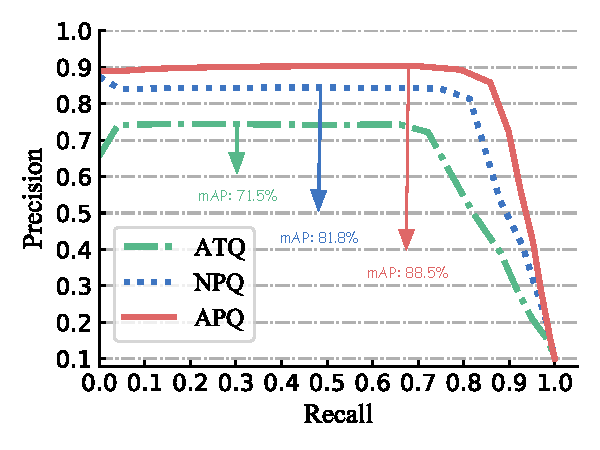
\includegraphics[height=5cm]{05/cifar_16b_anno.pdf}
    \caption{16位哈希码下在\textbf{CIFAR-10}上各种方法的\textbf{PR}曲线}
  \end{subfigure}
  \hspace{1cm}
  \begin{subfigure}{0.45\textwidth}
    \centering
    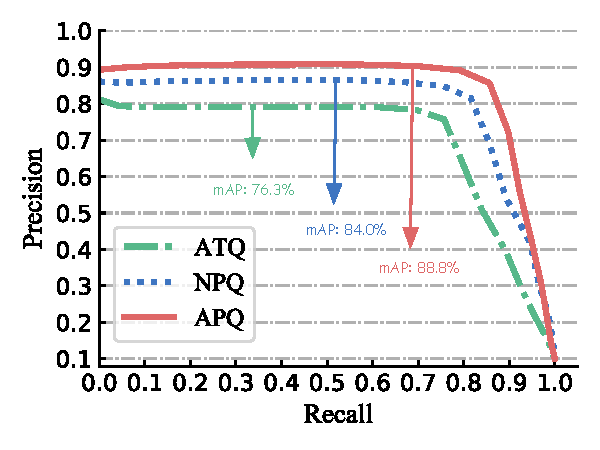
\includegraphics[height=5cm]{05/cifar_32b_anno.pdf}
    \caption{32位哈希码下在\textbf{CIFAR-10}上各种方法的\textbf{PR}曲线}
  \end{subfigure}
  \hspace{1cm}
  \begin{subfigure}{0.45\textwidth}
    \centering
    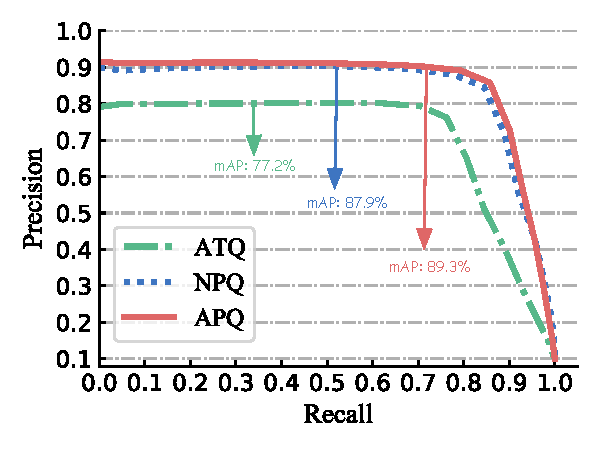
\includegraphics[height=5cm]{05/cifar_64b_anno.pdf}
    \caption{64位哈希码下在\textbf{CIFAR-10}上各种方法的\textbf{PR}曲线}
  \end{subfigure}
  \hspace{1cm}
  \begin{subfigure}{0.45\textwidth}
    \centering
    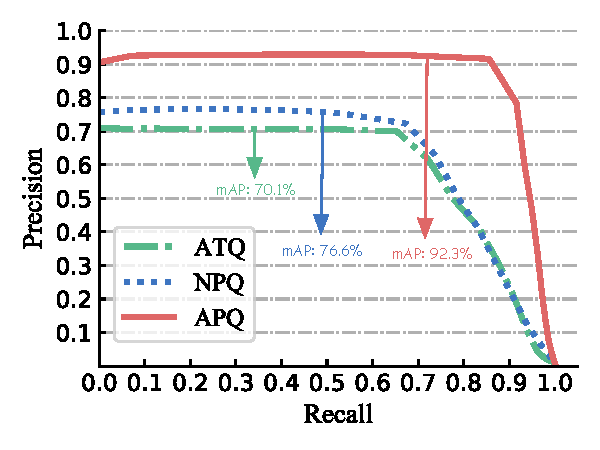
\includegraphics[height=5cm]{05/imagenet_16b_anno.pdf}
    \caption{16位哈希码下在\textbf{IMAGENET}上各种方法的\textbf{PR}曲线}
  \end{subfigure}
  \hspace{1cm}
  \begin{subfigure}{0.45\textwidth}
    \centering
    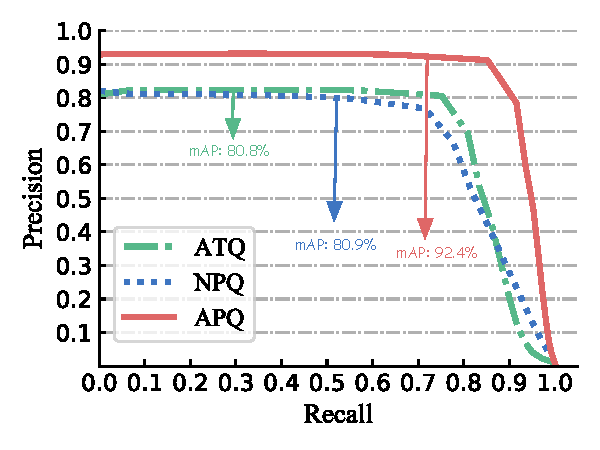
\includegraphics[height=5cm]{05/imagenet_32b_anno.pdf}
    \caption{32位哈希码下在\textbf{IMAGENET}上各种方法的\textbf{PR}曲线}
  \end{subfigure}
  \hspace{1cm}
  \begin{subfigure}{0.45\textwidth}
    \centering
    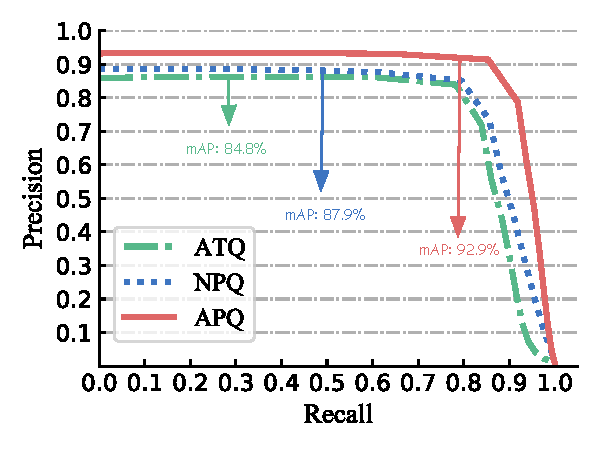
\includegraphics[height=5cm]{05/imagenet_64b_anno.pdf}
    \caption{64位哈希码下在\textbf{IMAGENET}上各种方法的\textbf{PR}曲线}
  \end{subfigure}
  \bicaption[各种量化损失函数在\textbf{CIFAR-10}和\textbf{IMAGENET}上的结果]{
      \textbf{APQ}量化损失和其他两种量化损失函数在\textbf{CIFAR-10}和\textbf{IMAGENET}数据集上的结果}{The experimental results on \textbf{CIFAR-10} and \textbf{IMAGENET} of \textbf{APQ} and other quantization losses.}
  \label{fig:abloss3}
\end{figure}

\subsection{消融实验}
在本小节, 我们对本章提出的\textbf{APQFormer}的每一个模块的作用进行了仔细的实验分析与研究。具体来说, 我们首先提供了详细的消融实验来研究主干神经网络来证实双支特征学习的必要性。随后, 我们将提出的量化学习损失函数\textbf{APQ} 和两个先进的量化损失函数进行实验来验证\textbf{APQ}损失函数的有效性。 最后, 我们将\textbf{APQ}和\textbf{APQ}基于的\textbf{FastAP}度量学习损失函数进行了比较, 证明非对称量化学习的有效性。\par
\textbf{主干网络的消融实验}: 我们设计了一个详尽的消融实验来验证本章中提出的主干网络的双支学习的有效性。具体来说, 我们设计了两种主干网路的变种:
\begin{enumerate}
    \item \textbf{APQFormer-C}: 一个只包含\textbf{C-branch}的\textbf{APQFormer}的变种。
    \item \textbf{APQFormer-F}: 一个只包含\textbf{F-branch}的\textbf{APQFormer}的变种。
\end{enumerate}
值得注意的是, 我们测量的这两个变种基于同等多的标准的Transformer block 并且其多头注意力的头数也一致。如表~\ref{table:abdtq}所示, 完整的模型~\textbf{APQFormer} 在两个数据集上以及三种不同的哈希长度上以较大幅度的性能差距明显超过其他两种变种。这证明了双支Vision Transformer的特征设计的有效性。 同时, 我们也能观察到~\textbf{APQFormer-F}变种在各种场景下性能优于\textbf{APQFormer-C}。这是由于其采取的图片分块的数量更大, 可以学到更加细粒度的特征。但是值得注意的是, 这也会导致计算量的显著增大。\par
\textbf{和其他的量化损失函数的对比}:  我们额外提供了实验分析证明我们提出的量化损失函数~\textbf{APQ}的有效性。我们和以下两种先进的量化损失函数进行了细致的比较:
\begin{enumerate}
    \item \textbf{ATQ} 是一个由Yu等人\cite{yu2018product}提出的非对称的三元量化损失函数。
    \item \textbf{NPQ} 是有Jang等人\cite{jang2020generalized}提出的用于半监督图像检索场景的n-pair 量化损失函数。
\end{enumerate}


实验结果如图~\ref{fig:abloss3}所示。很明显, 我们提出的量化损失函数~\textbf{APQ}可以以大幅度性能优势领先其余两种量化损失函数。特别来说, 在\textbf{IMAGENET}数据集上, 我们在\textbf{mAP}指标上, 分别超越了\textbf{ATQ} 和\textbf{NPQ} 平均 \textbf{$14.01$}\% 和 \textbf{$10.75$}\%。 在 \textbf{CIFAR-10}数据集上, \textbf{APQ} 也以大幅度领先于\textbf{ATQ} 和 \textbf{NPQ}。在16位哈希码长度下, \textbf{APQ}取得了 $\textbf{88.5\%}$ \textbf{mAP}, 分别超出\textbf{ATQ} 和 \textbf{NPQ} $17.0\%$ 和 $6.7 \%$。在32位哈希码长度下, \textbf{APQ}取得了 $\textbf{88.8\%}$ \textbf{mAP}, 分别超出\textbf{ATQ} 和 \textbf{NPQ} $12.5\%$ 和 $4.8 \%$。同时, 在图~\ref{fig:abloss3}中, 我们也可以观察到 \textbf{APQ}的 \textbf{PR} 曲线始终在其余两个量化损失函数对应的曲线之上, 这进一步证实了我们的损失函数的有效性。\par
\begin{figure}[!htp]
  \centering
  \begin{subfigure}{0.45\textwidth}
    \centering
    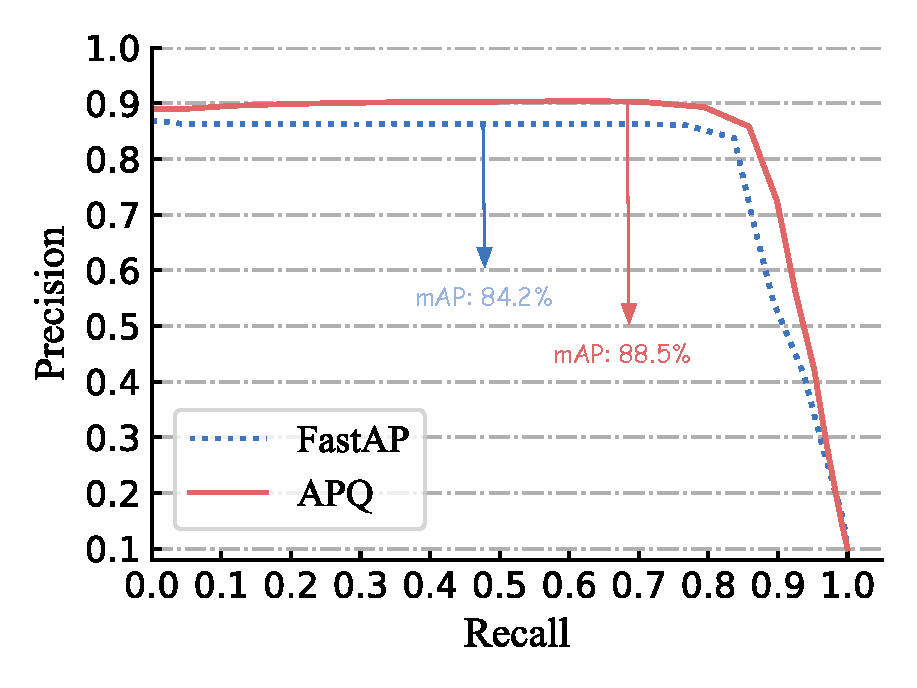
\includegraphics[height=5cm]{05/ablation_cifar_16b_anno.pdf}
    \caption{16位哈希码下在\textbf{CIFAR-10}上\textbf{APQ}和\textbf{FastAP}的性能比较}
  \end{subfigure}
  \hspace{1cm}
  \begin{subfigure}{0.45\textwidth}
    \centering
    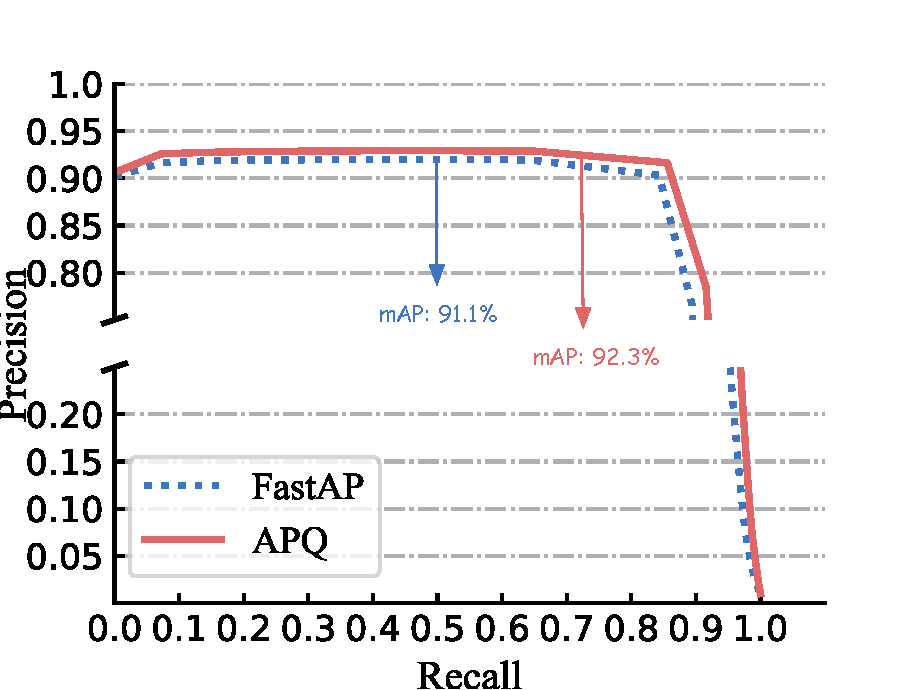
\includegraphics[height=5cm]{05/absym_imagenet_16b_anno.pdf}
    \caption{16位哈希码下在\textbf{IMAGENET}上\textbf{APQ}和\textbf{FastAP}的性能比较}
  \end{subfigure}
  \hspace{1cm}
  \bicaption[\textbf{FastAP}和\textbf{APQ}量化损失函数的性能比较]{
      \textbf{APQ}和\textbf{FastAP}在两个数据集上性能比较的结果}{The experimental results on two datasets  of \textbf{APQ} and \textbf{FastAP} }
  \label{fig:abapfast}
\end{figure}

\begin{figure}[!htp]
  \centering
  \begin{subfigure}{0.45\textwidth}
    \centering
    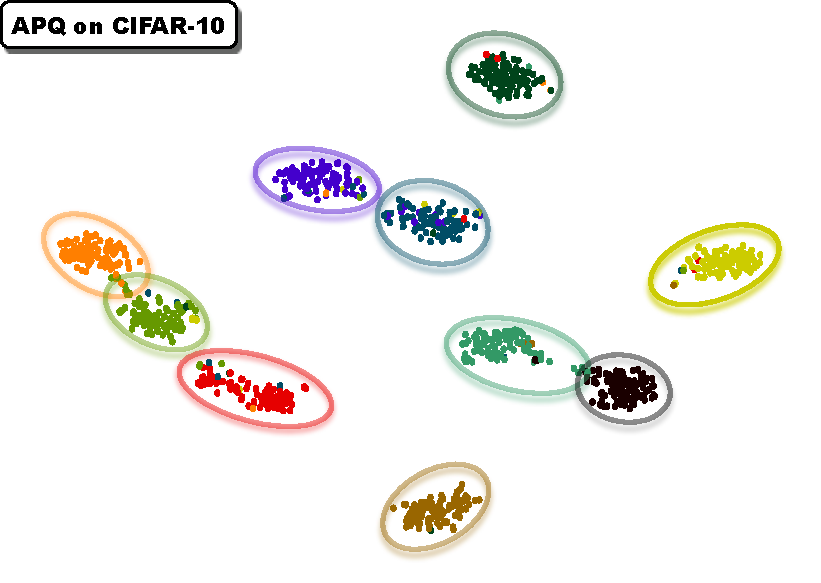
\includegraphics[height=5cm]{05/apq_tsne_anno.pdf}
    \caption{16位哈希码下在\textbf{CIFAR-10}上\textbf{APQ}的深度特征t-SNE可视化}
  \end{subfigure}
  \hspace{1cm}
  \begin{subfigure}{0.45\textwidth}
    \centering
    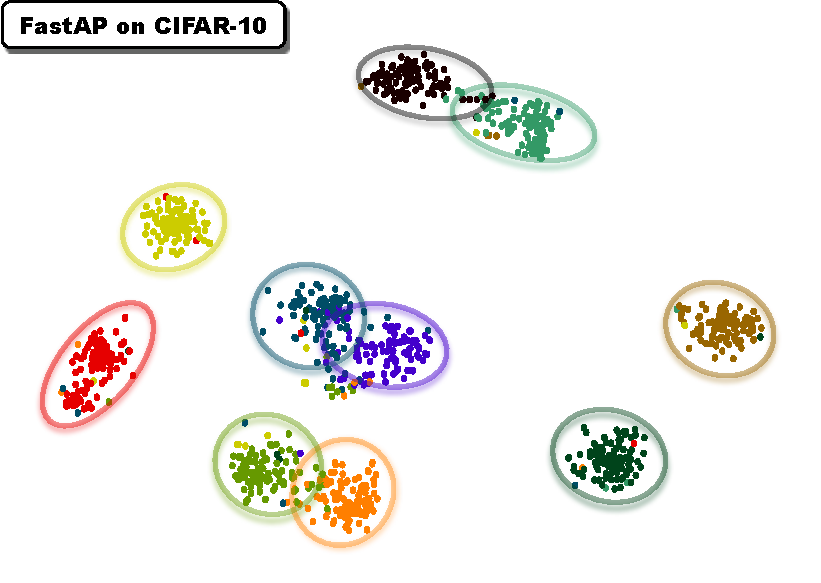
\includegraphics[height=5cm]{05/fastap_tsne_anno.pdf}
    \caption{16位哈希码下在\textbf{IMAGENET}上\textbf{FastAP}的深度特征t-SNE可视化}
  \end{subfigure}
  \bicaption[\textbf{FastAP}和\textbf{APQ}的深度特征t-SNE可视化图对比]{
      \textbf{APQ}和\textbf{FastAP}在\textbf{CIFAR-10}上的深度特征可视化}{The t-SNE Visualization of deep features learned by \textbf{APQ} and \textbf{FastAP} on \textbf{CIFAR-10}}
  \label{fig:abapfast1}
\end{figure}

\textbf{APQ Vs FastAP}。为了进一步分析\textbf{APQ}的性能, 我们进行了一系列其他的实验来将\textbf{APQ}和\textbf{FastAP}进行比较。\textbf{FastAP}~~\cite{cakir2019deep}是设计用来进行通用的度量学习的损失函数。 我们在图~\ref{fig:abapfast}中画出来\textbf{PR} 曲线和~\textbf{mAP}的结果。同时, 我们进一步画出两个损失函数学习到的深度特征的 t-SNE 可视化图~\ref{fig:abapfast1}。很明显, \textbf{APQ} 在\textbf{PR} 曲线和~\textbf{mAP}上持续性的超越了\textbf{FastAP}。同时, 如图~\ref{fig:abapfast1}所示, \textbf{APQ}可以学习到更加紧凑可以区分的深度特征。 
\section{总结}
本章提出了第一个基于Vision Transformer的端到端的乘积量化框架-\textbf{APQFormer}。提出的\textbf{APQFormer}包含了一个双支的基于Vision Transformer的量化主干网络~\textbf{DTQN}。 其可以同时进行多尺度特征学习以及端到端的乘积量化学习。 对于相似度保留的监督训练, 我们提出了一个新型的量化损失函数\textbf{APQ} 直接优化评估指标\textbf{mAP}。我们在标准的数据集上进行了大量的实验。实验结果证实了本章提出的算法的有效性以及和其他基于传统卷积神经网络的量化方法相比较的优越性。